\subsection{Le dipôle court: $l \ll \lambda$}
Le gain de l'antenne dans le plan E est représenté dans la figure \ref{fig:gain21}.
\begin{figure}[htbp]
  \centering
  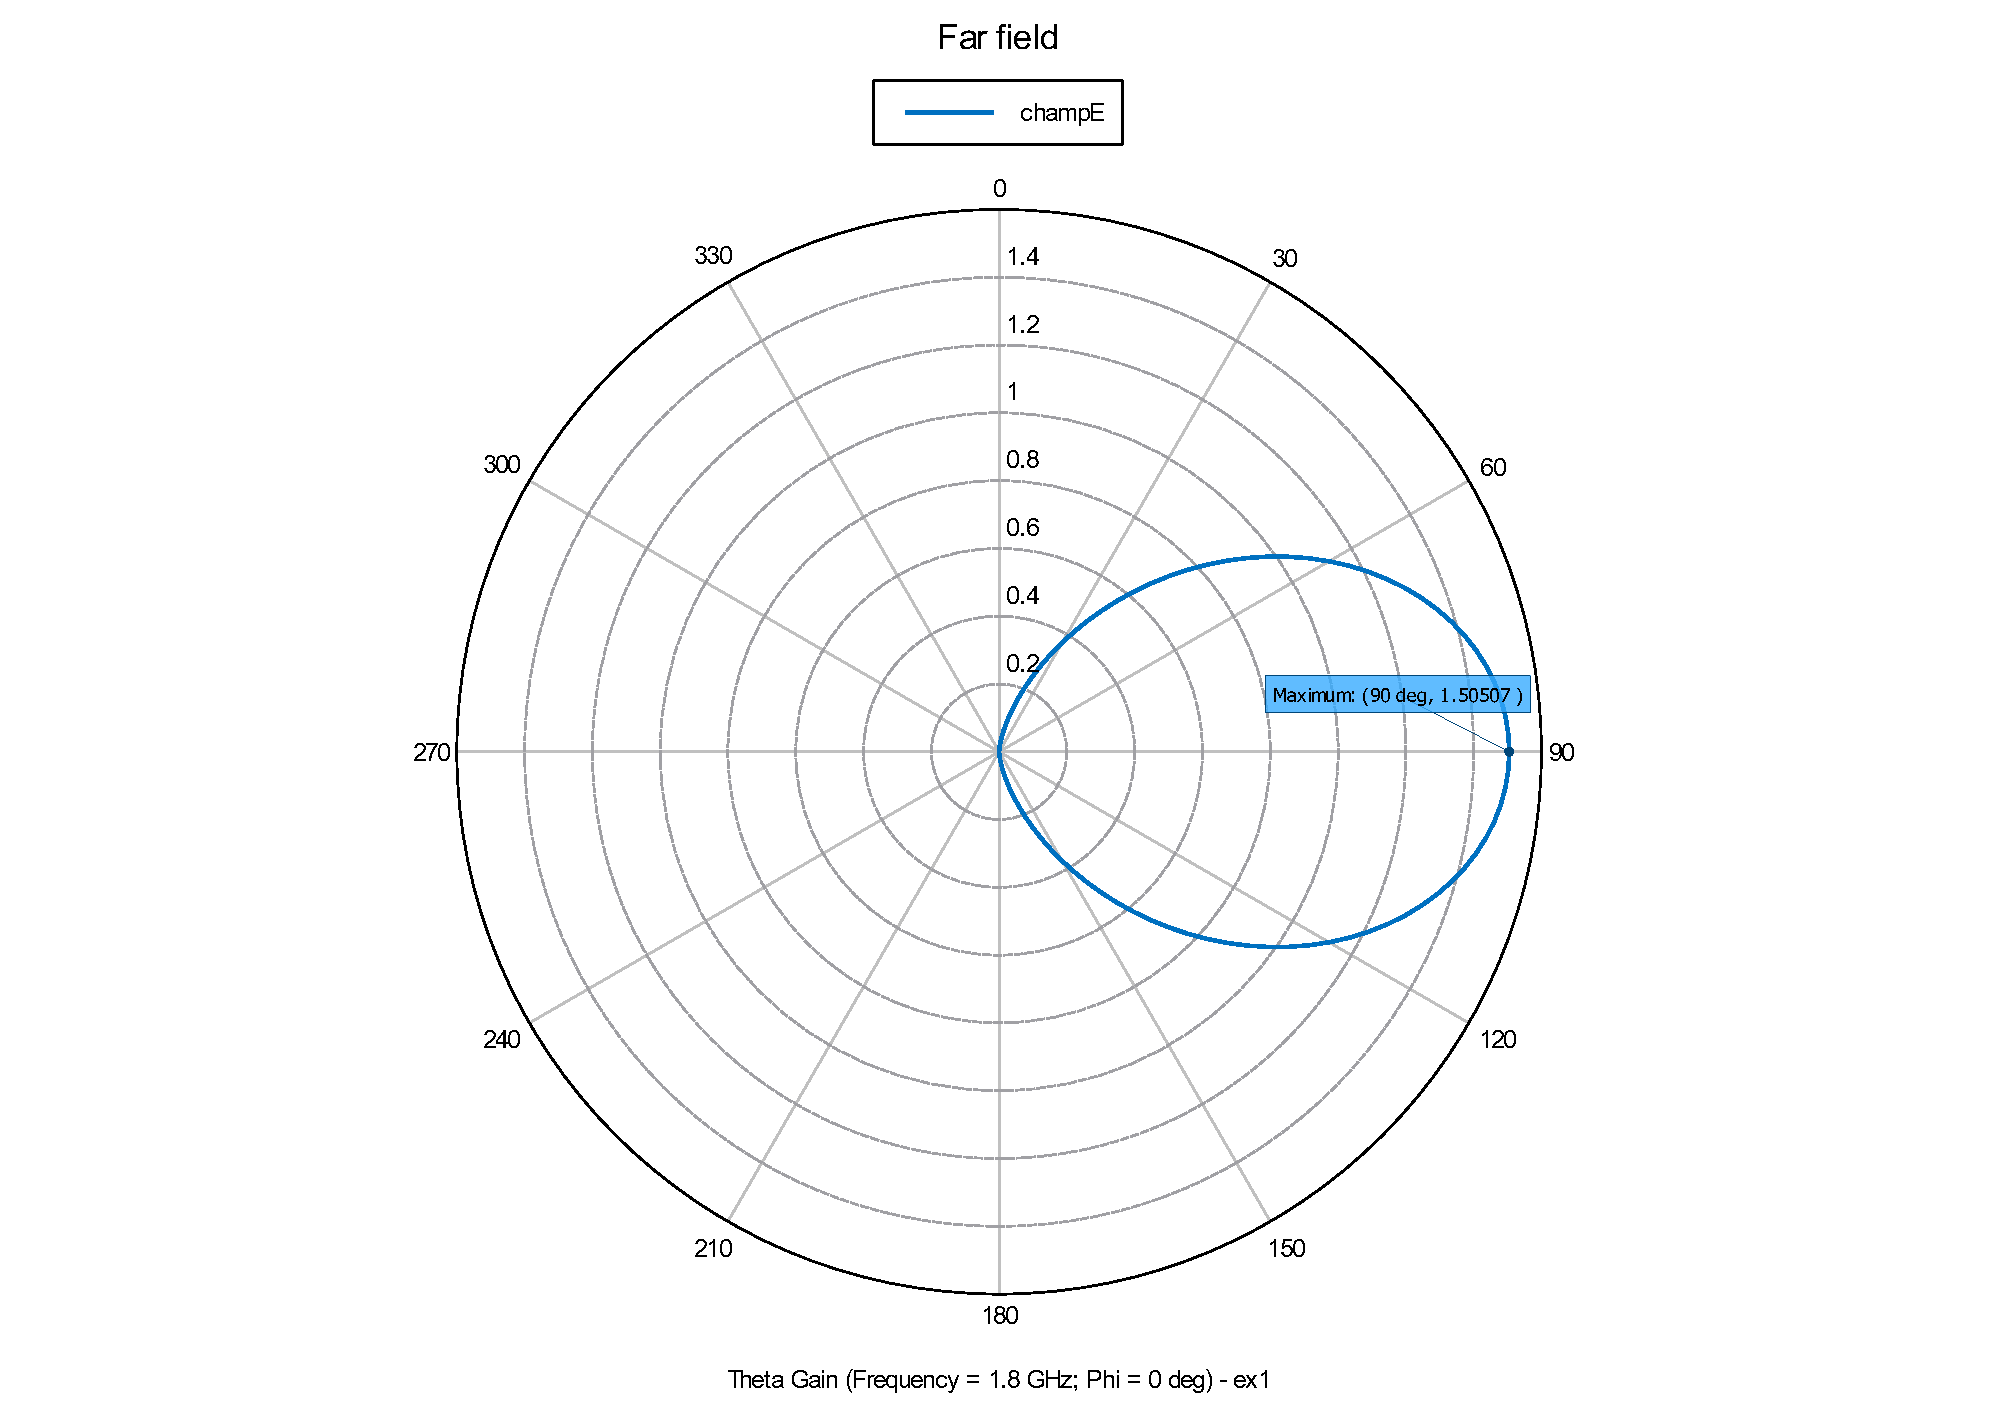
\includegraphics[width=\textwidth]{gain21.pdf}
  \caption{Diagramme de rayonnement du dipôle court dans le plan E.\label{fig:gain21}}
\end{figure}
Le gain n'est pas représenté pour $\SI{180}{\degree}<\theta<\SI{360}{\degree}$, ce qui n'est pas important puisque l'on sait que le problème présente une symétrie cylindrique. Pour la même raison, les diagrammes dans le plan H ne sont pas donnés ici, mais se déduisent logiquement de la figure \ref{fig:gain21}: le gain est indépendant de $\phi$. Sa composante $\theta$ vaut le gain maximal du diagramme de rayonnement dans le plan E, et sa composante $\phi$ vaut $0$.

Sur la figure \ref{fig:gain21}, on lit un gain maximal de $\num{1.51} = \SI{1.79}{\deci\bel}$, ce qui est légèrement supérieur à la valeur $\frac{3}{2} = \SI{1.76}{\deci\bel}$ prédite par l'approximation du dipôle de Hertz. Ceci est logique puisque la directivité maximale augmente lorsqu'on augmente la longueur du dipôle.

La résistance de rayonnement est représentée en fonction de la fréquence à la figure \ref{fig:Rar21}.
\begin{figure}[htbp]
  \centering
  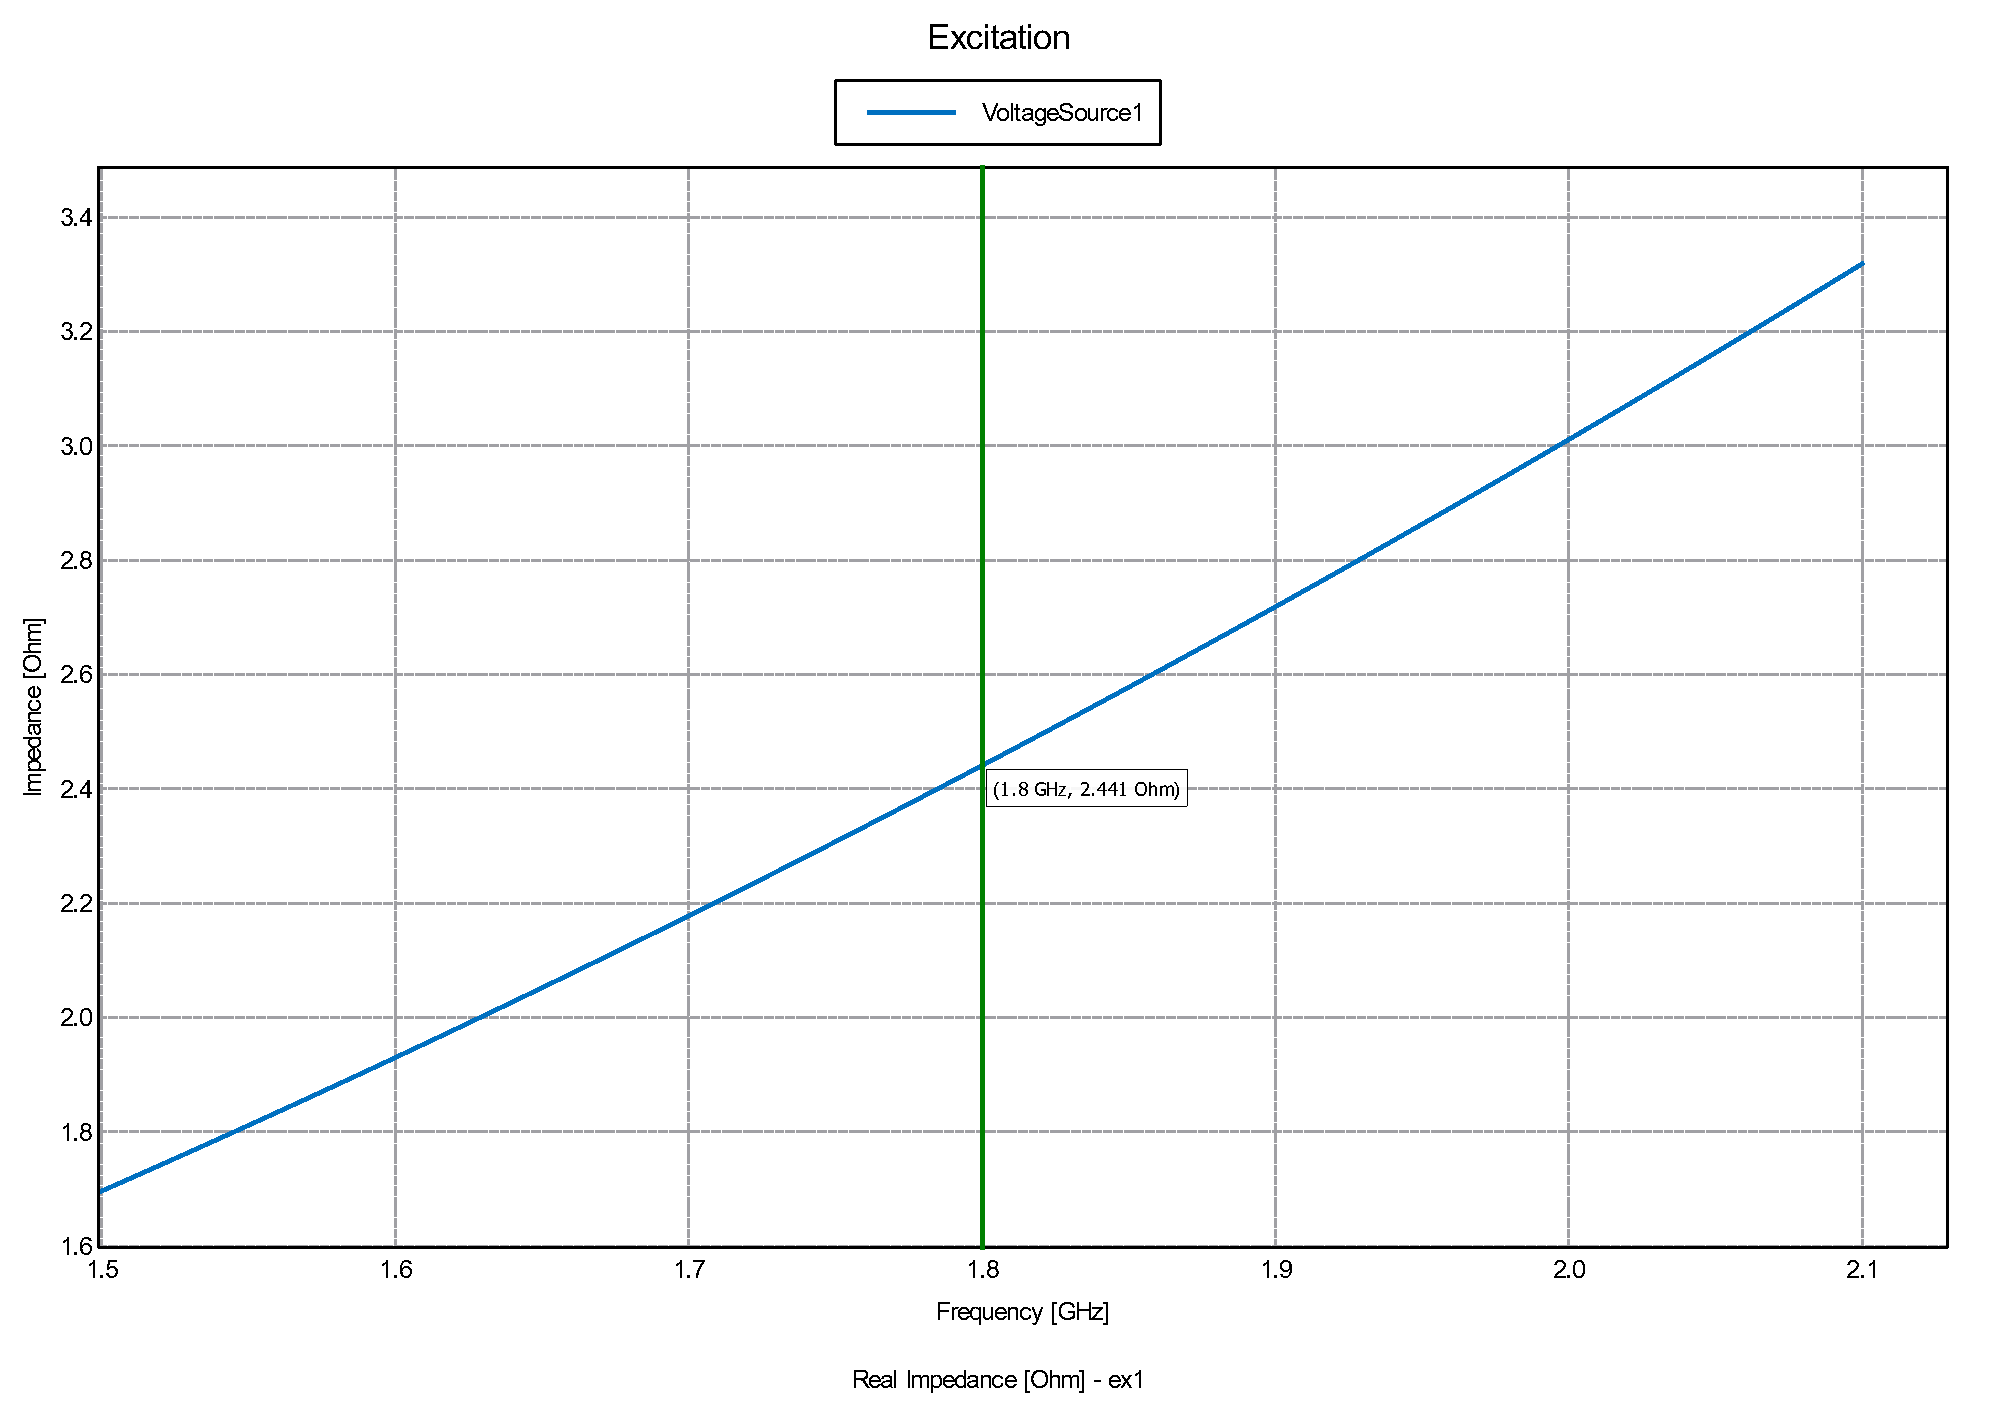
\includegraphics[width=\textwidth]{Rar21.pdf}
  \caption{Résistance de rayonnement du dipôle court en fonction de la fréquence.\label{fig:Rar21}}
\end{figure}
Puisque le fil est modélisé par un conducteur parfait et que les connexions ne sont pas prises en compte, la résistance ohmique est considérée comme nulle. Sur la figure \ref{fig:Rar21}, on lit $R_{ar} = \SI{2.44}{\ohm}$ pour $f = \SI{1.8}{\giga\hertz}$, ce qui est très inférieur à la valeur $R_{ar} = 80 \left (\frac{\pi l}{\lambda} \right ) ^2 = \SI{7.90}{\ohm}$ prédite par l'approximation de l'élément de courant.

A partir de cette valeur, on obtient la fraction de puissance consommée par l'antenne en calculant d'abord $\Gamma_L$ puis en utilisant la relation \ref{eqn:puissance délivrée}.
\begin{align*}
\Gamma_L = \frac{Z_L - Z_c}{Z_L + Z_c} &= 0.91\numberthis\label{eqn:reflect}\\
\frac{P_L}{P_{in}} &= \SI{17.7}{\percent}
\end{align*}
L'adaptation d'impédance est donc très mauvaise. Ceci peut-être résolu en utilisant un dipôle demi-onde, comme nous le verrons dans la prochaine section.

\subsection{Le dipôle demi-onde: $l = \frac{\lambda}{2}$}
\label{subsec:demionde}
Le gain dans le plan E est représenté dans un diagramme polaire à la figure \ref{fig:gain22}.
\begin{figure}[htbp]
  \centering
  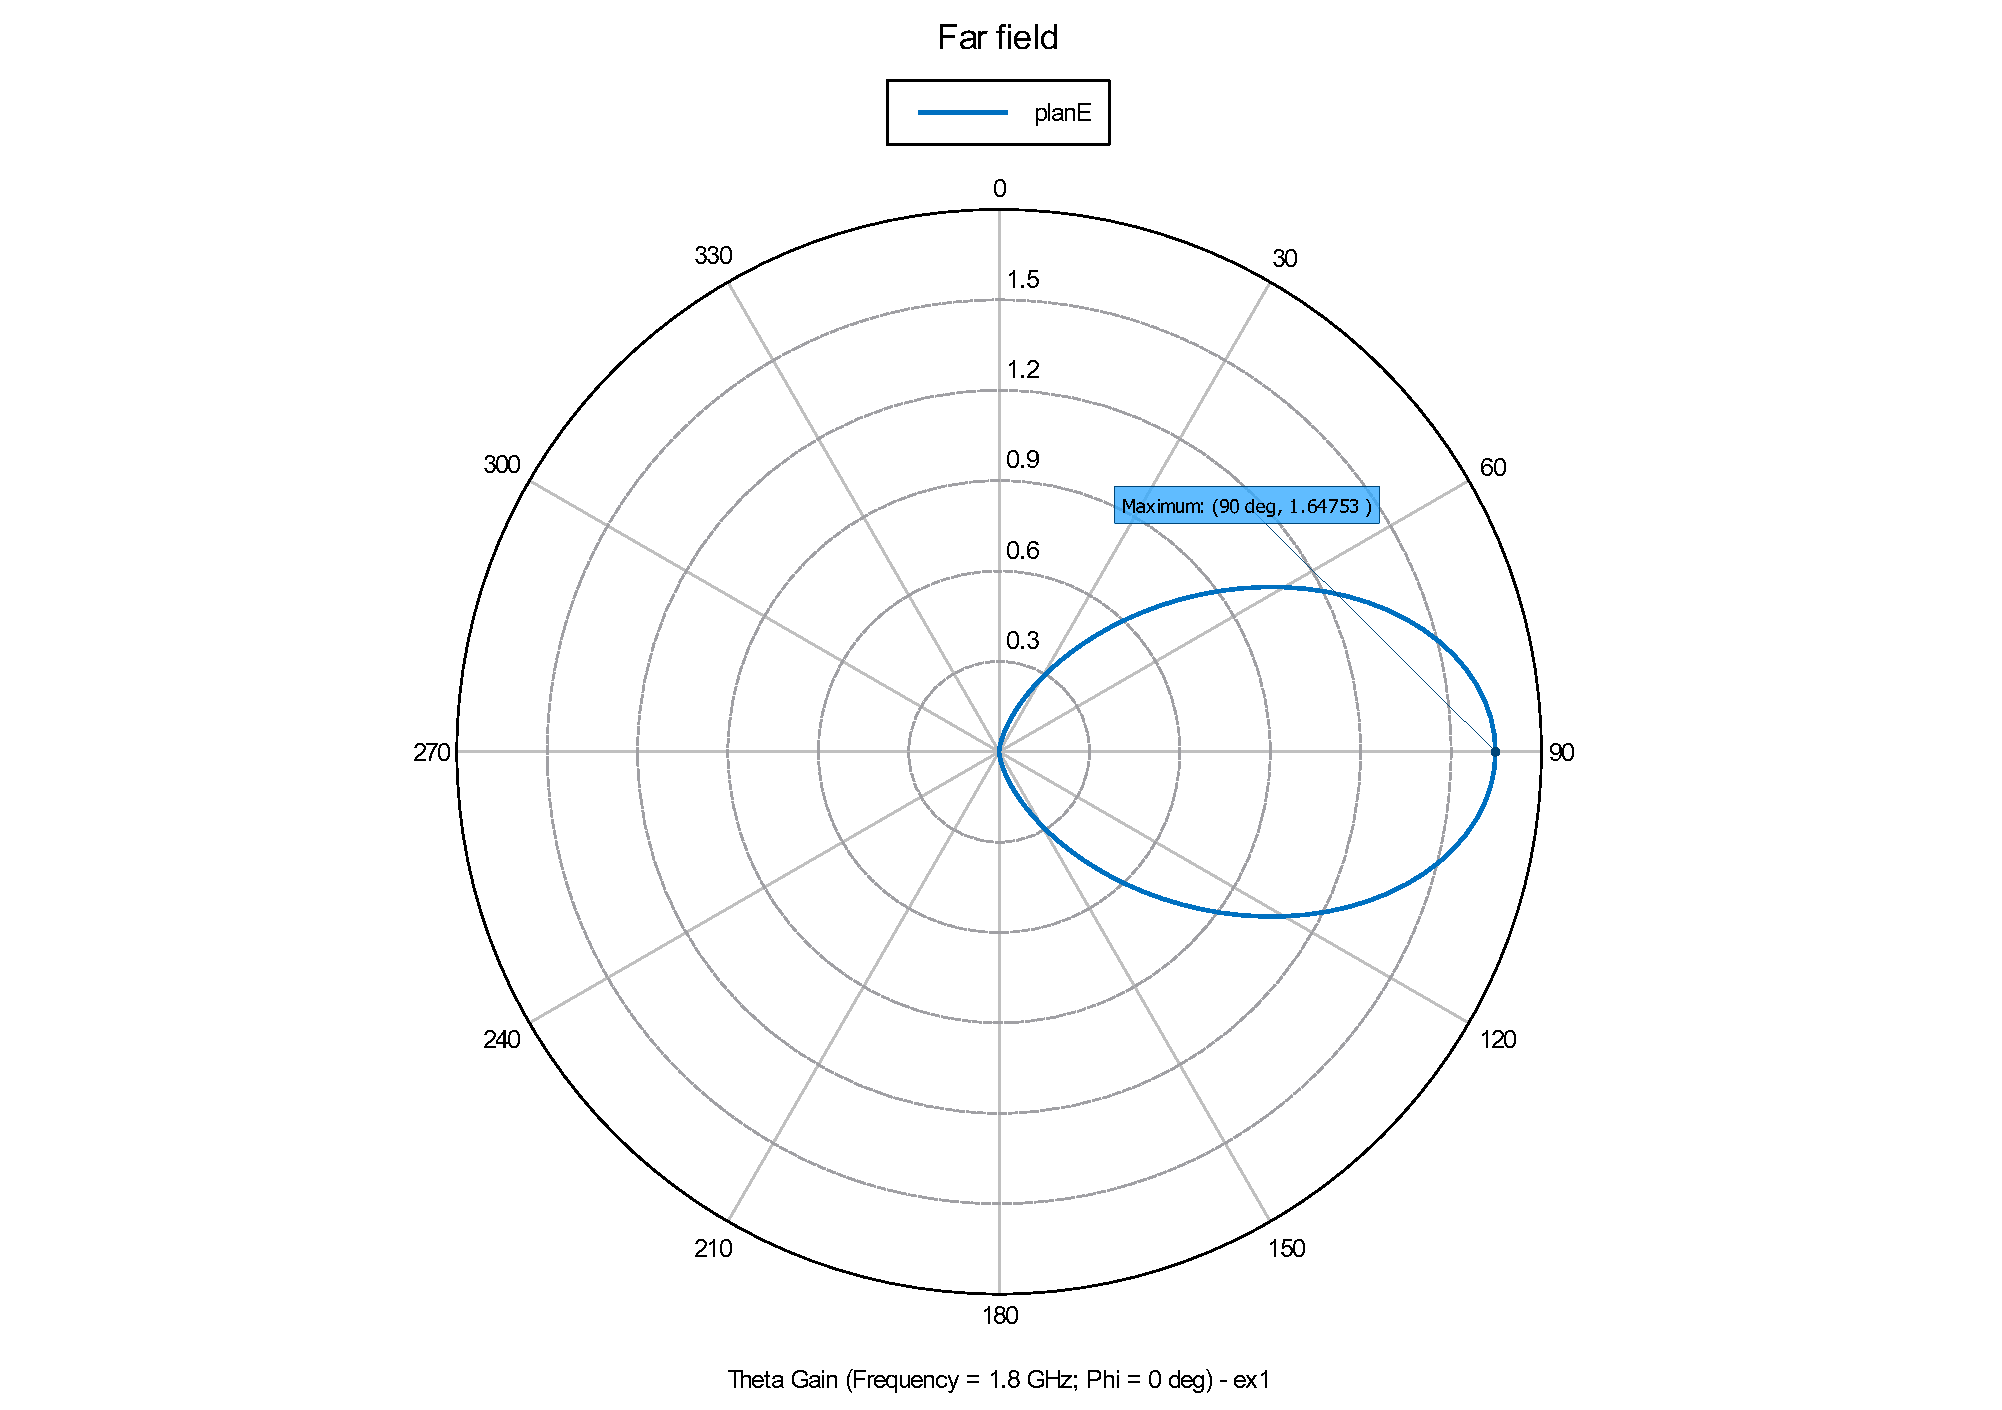
\includegraphics[width = \textwidth]{Rar22.pdf}
  \caption{Diagramme de rayonnement du dipôle demi-onde dans le plan E.\label{fig:gain22}}
\end{figure}
Les propriétés de symétrie de la figure \ref{fig:gain21} s'appliquent toujours. On lit sur le diagramme de rayonnement un gain maximal de \num{1.65}, ce qui est légèrement inférieur à la valeur de \num{1.7} prédite avec l'approximation
\[\left ( \frac{\cos(\frac{\pi}{2}\cos\theta)}{\sin\theta} \right ) ^2 \simeq \sin^3 \theta\]

Sur la figure \ref{fig:Z22},
\begin{figure}[htbp]
  \centering
  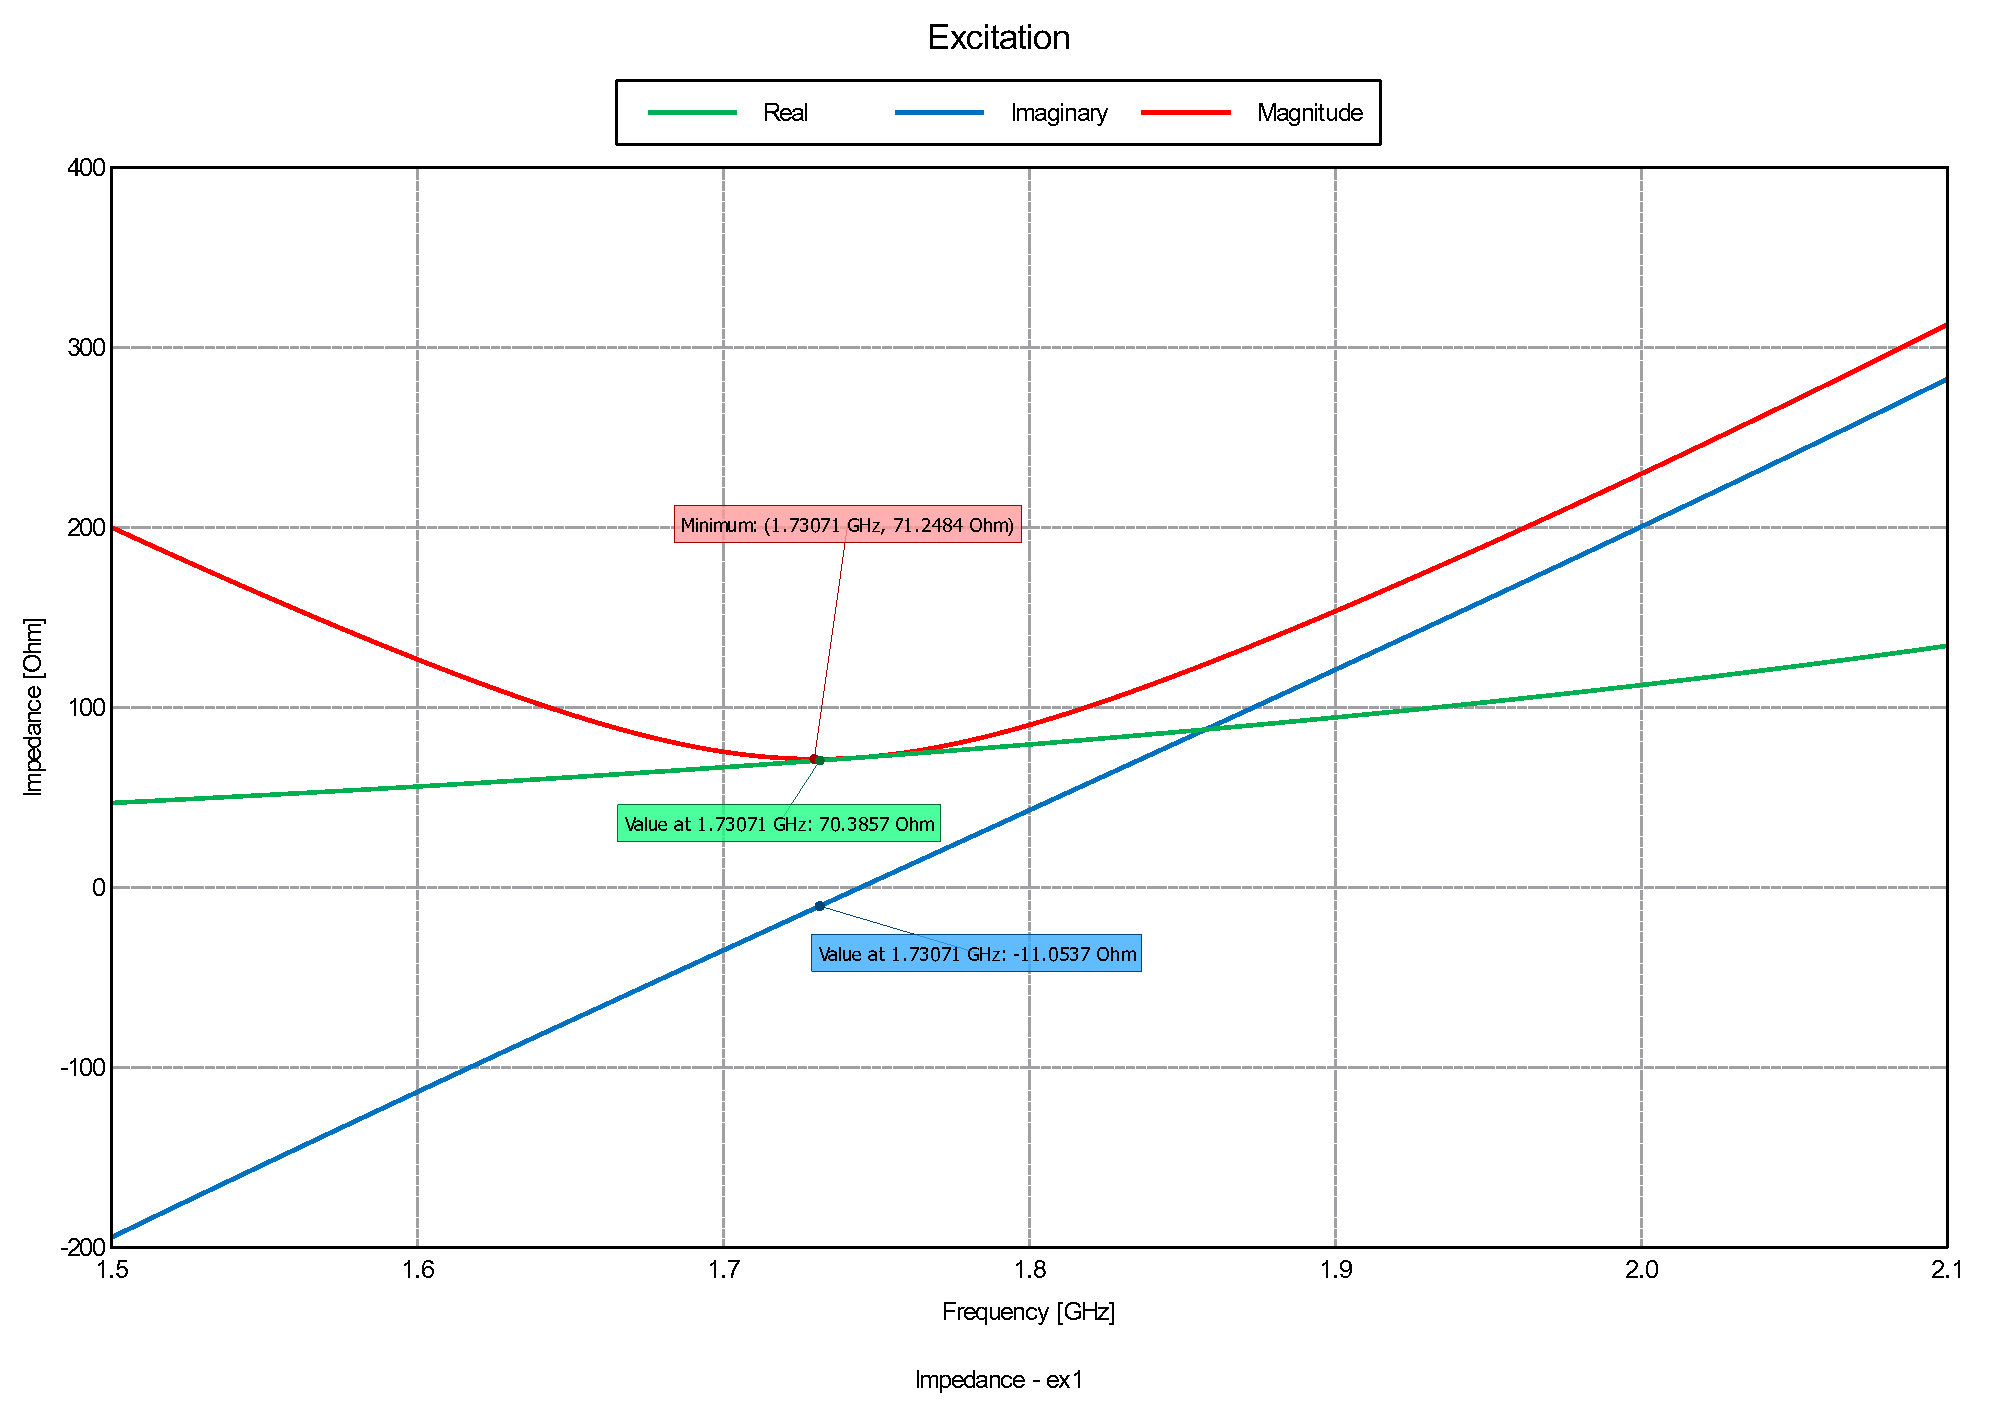
\includegraphics[width = \textwidth]{Z22.pdf}
  \caption{Parties réelle et imaginaire et module de l'impédance de l'antenne en fonction de la fréquence.\label{fig:Z22}}
\end{figure}
on constate que la partie imaginaire de l'impédance croît linéairement avec la fréquence, et ce beaucoup plus rapidement que la partie réelle qui peut être considérée comme quasi constante. De plus, comme la partie imaginaire évolue d'une valeur négative vers une valeur positive, le module de l'impédance n'est lui pas monotone et présente un minimum qui est approximativement donné par le zéro de la partie imaginaire. Sur la figure \ref{fig:Z22}, ce point se situe à \SI{1.73}{\giga\hertz}. Nous allons maintenant essayer de le déplacer à \SI{1.8}{\giga\hertz} en modifiant la longueur du dipôle.

Ceci est fait à la figure \ref{fig:Z022}.
\begin{figure}[htbp]
  \centering
  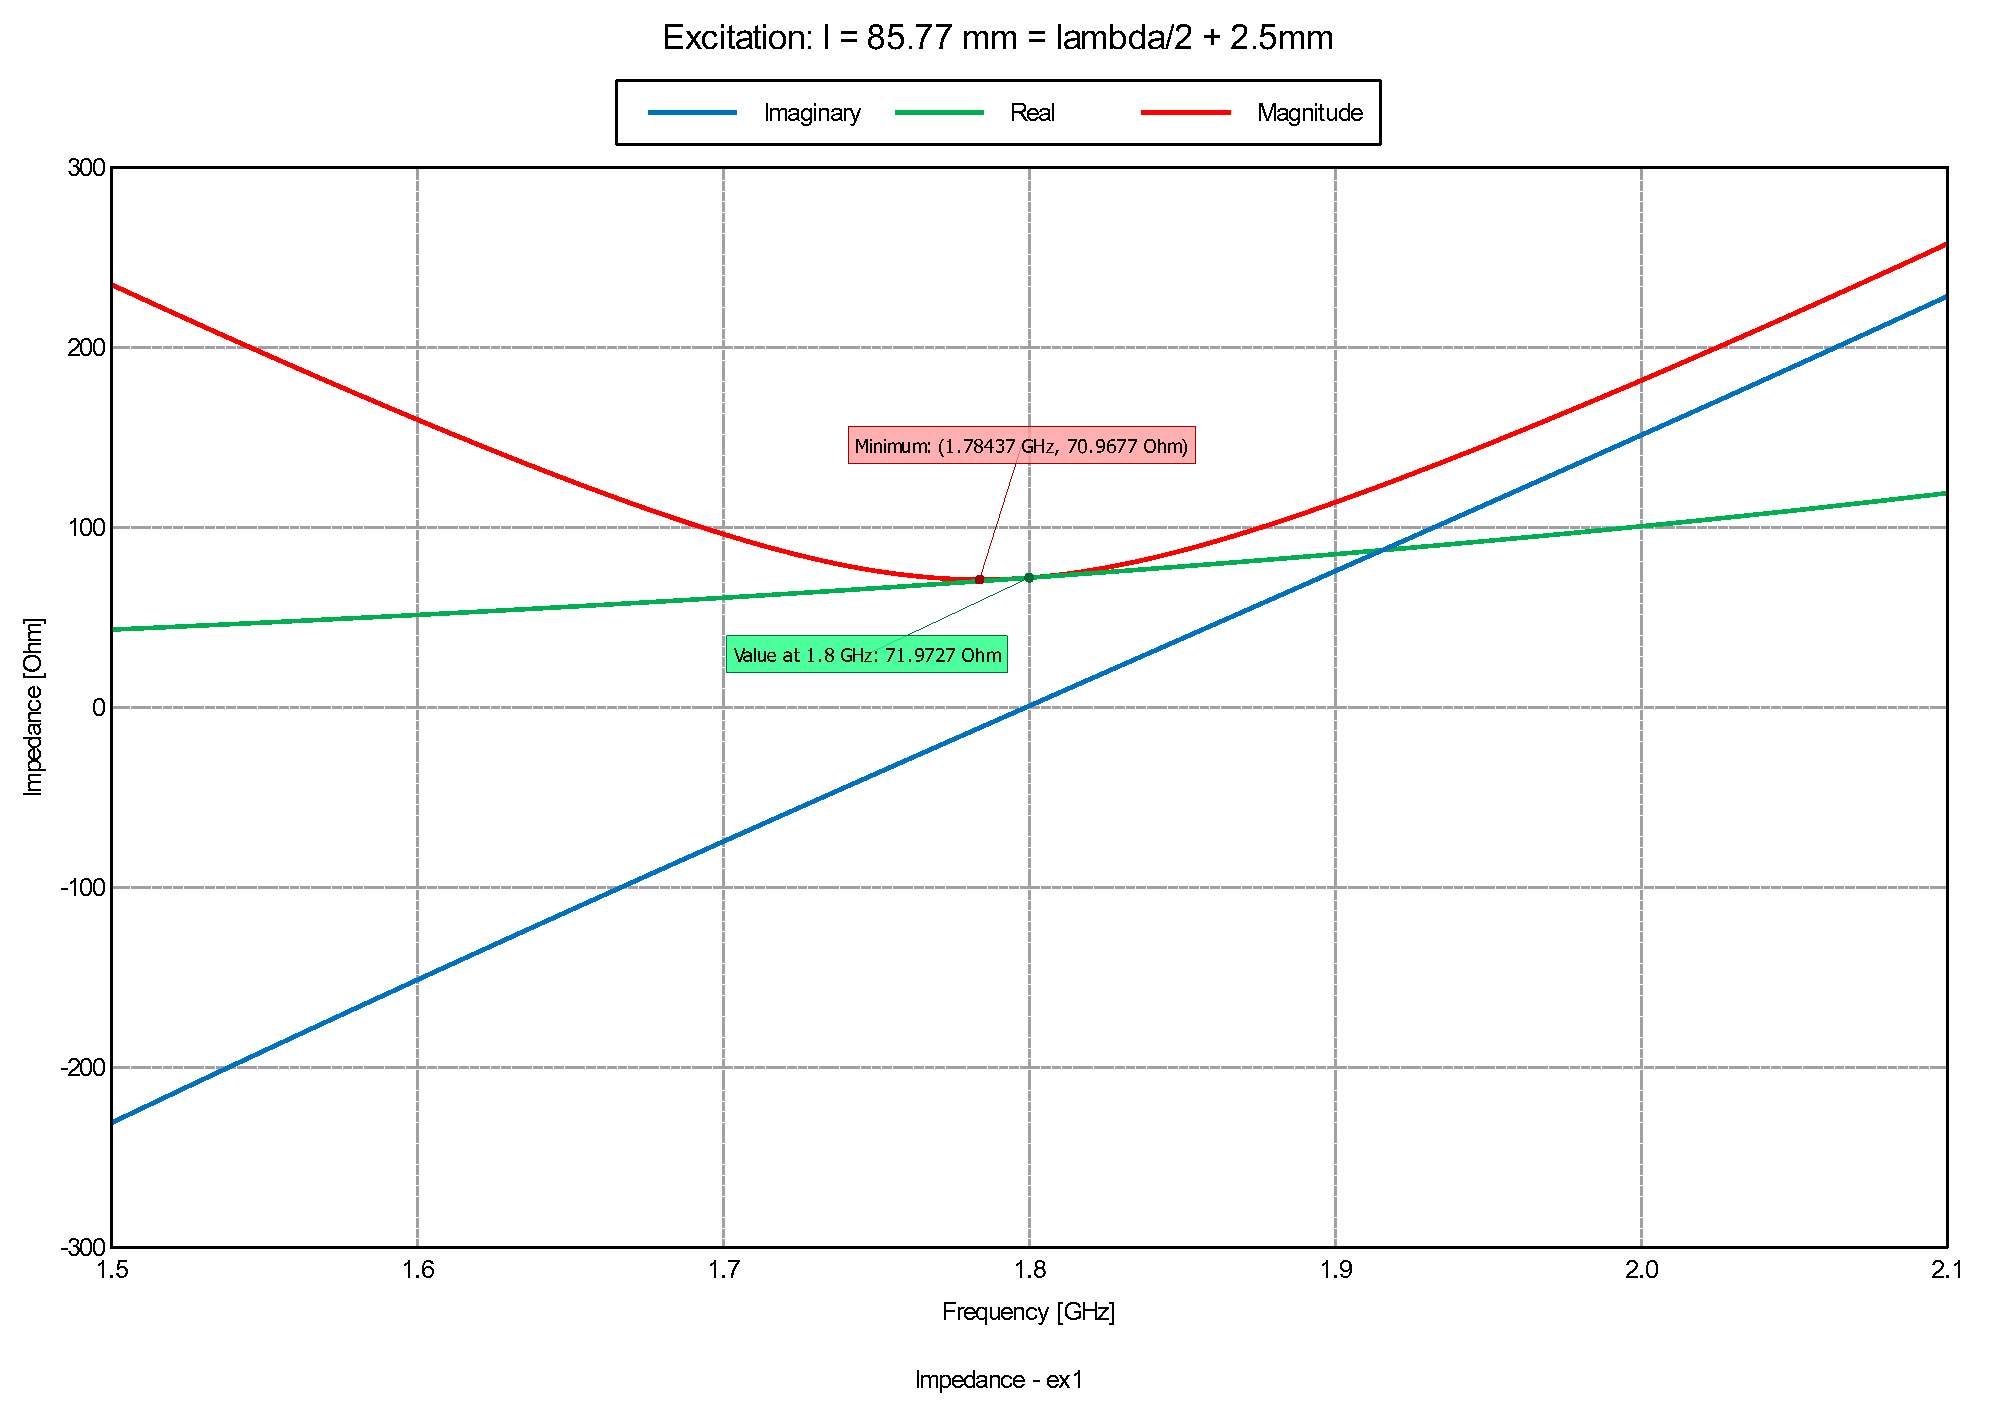
\includegraphics[width = \textwidth]{Z022.pdf}
  \caption{Parties réelle et imaginaire et module de l'impédance de l'antenne adaptée pour \SI{1.8}{\giga\hertz} en fonction de la fréquence.\label{fig:Z022}}
\end{figure}
La partie imaginaire de l'impédance s'annule bien en $f = \SI{1.8}{\giga\hertz}$ et le module de l'impédance de rayonnement est donc proche de son minimum à cette fréquence.

En utilisant la relation \ref{eqn:reflect}, on obtient $\Gamma_L = 0.027 = \SI{-31.2}{\deci\bel}$ pour $Z_c = \SI{75}{\ohm}$. Ceci est confirmé par la simulation, comme le montre la figure \ref{fig:gamma22}.
\begin{figure}[htbp]
  \centering
  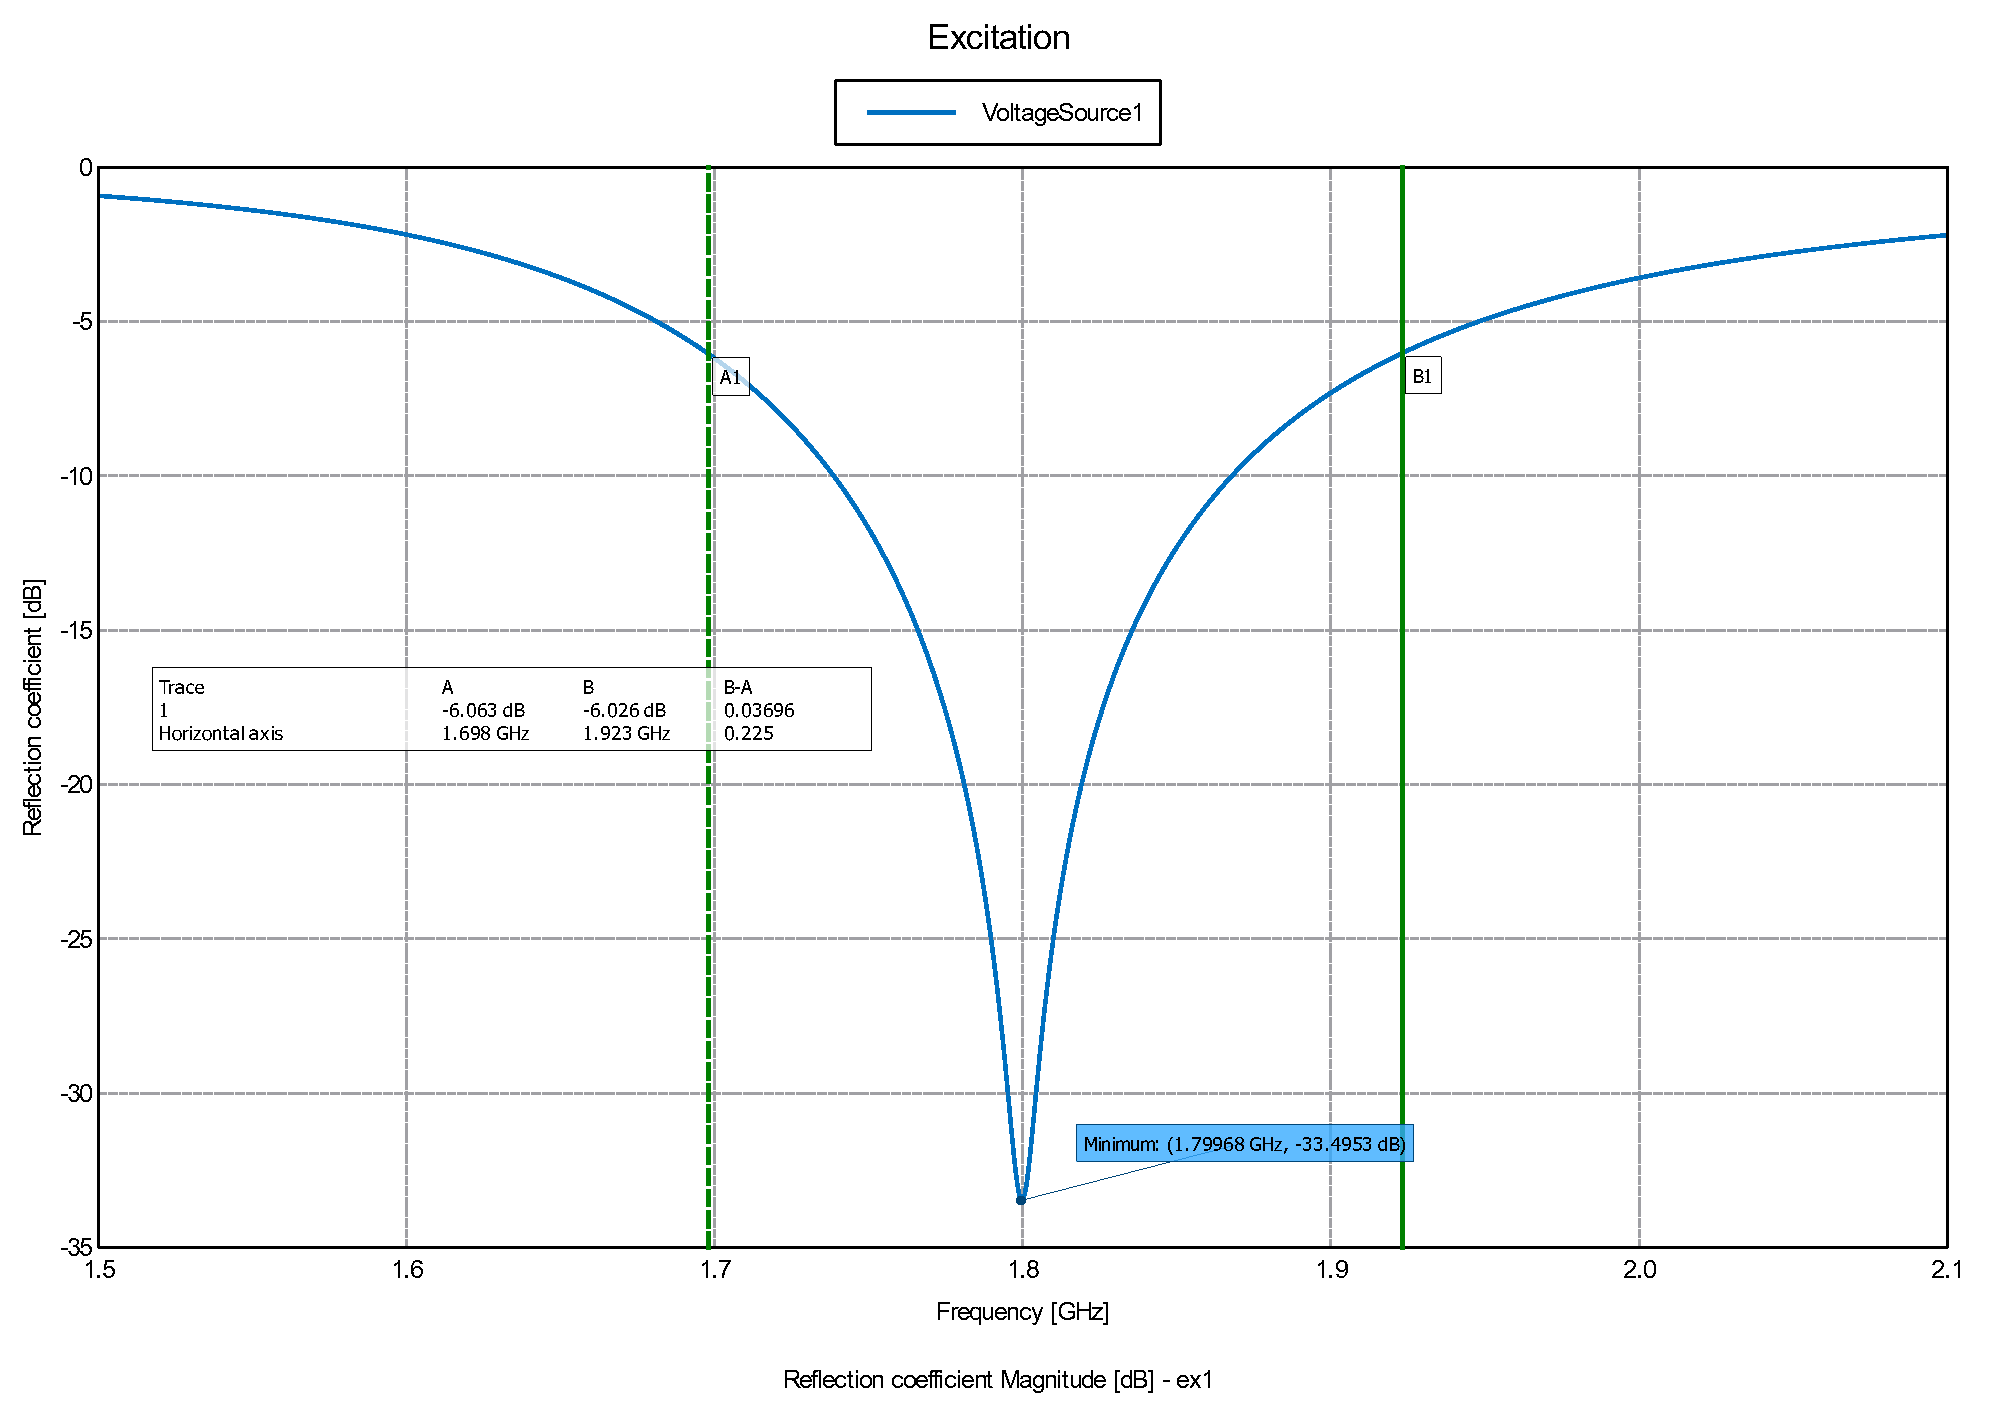
\includegraphics[width = \textwidth]{gamma22.pdf}
  \caption{$\Gamma_L$ de l'antenne dipôle adaptée pour \SI{1.8}{\giga\hertz} en fonction de la fréquence.\label{fig:gamma22}}
\end{figure}
De ce coefficient de réflexion on tire la fraction de puissance consommée à l'antenne par la relation \ref{eqn:puissance délivrée}.
\[
  \frac{P_L}{P_{in}} = \SI{99.9}{\percent}
\]

Jusqu'à présent, nous avons travaillé avec un diamètre de fil de $0.00001 \lambda$. Lorsqu'on multiplie ce diamètre par 50, on constate que la fréquence de résonance est légèrement diminuée, mais surtout que la bande passante est plus que doublée, comme le montre la figure \ref{fig:gamma5022}.
\begin{figure}[htbp]
  \centering
  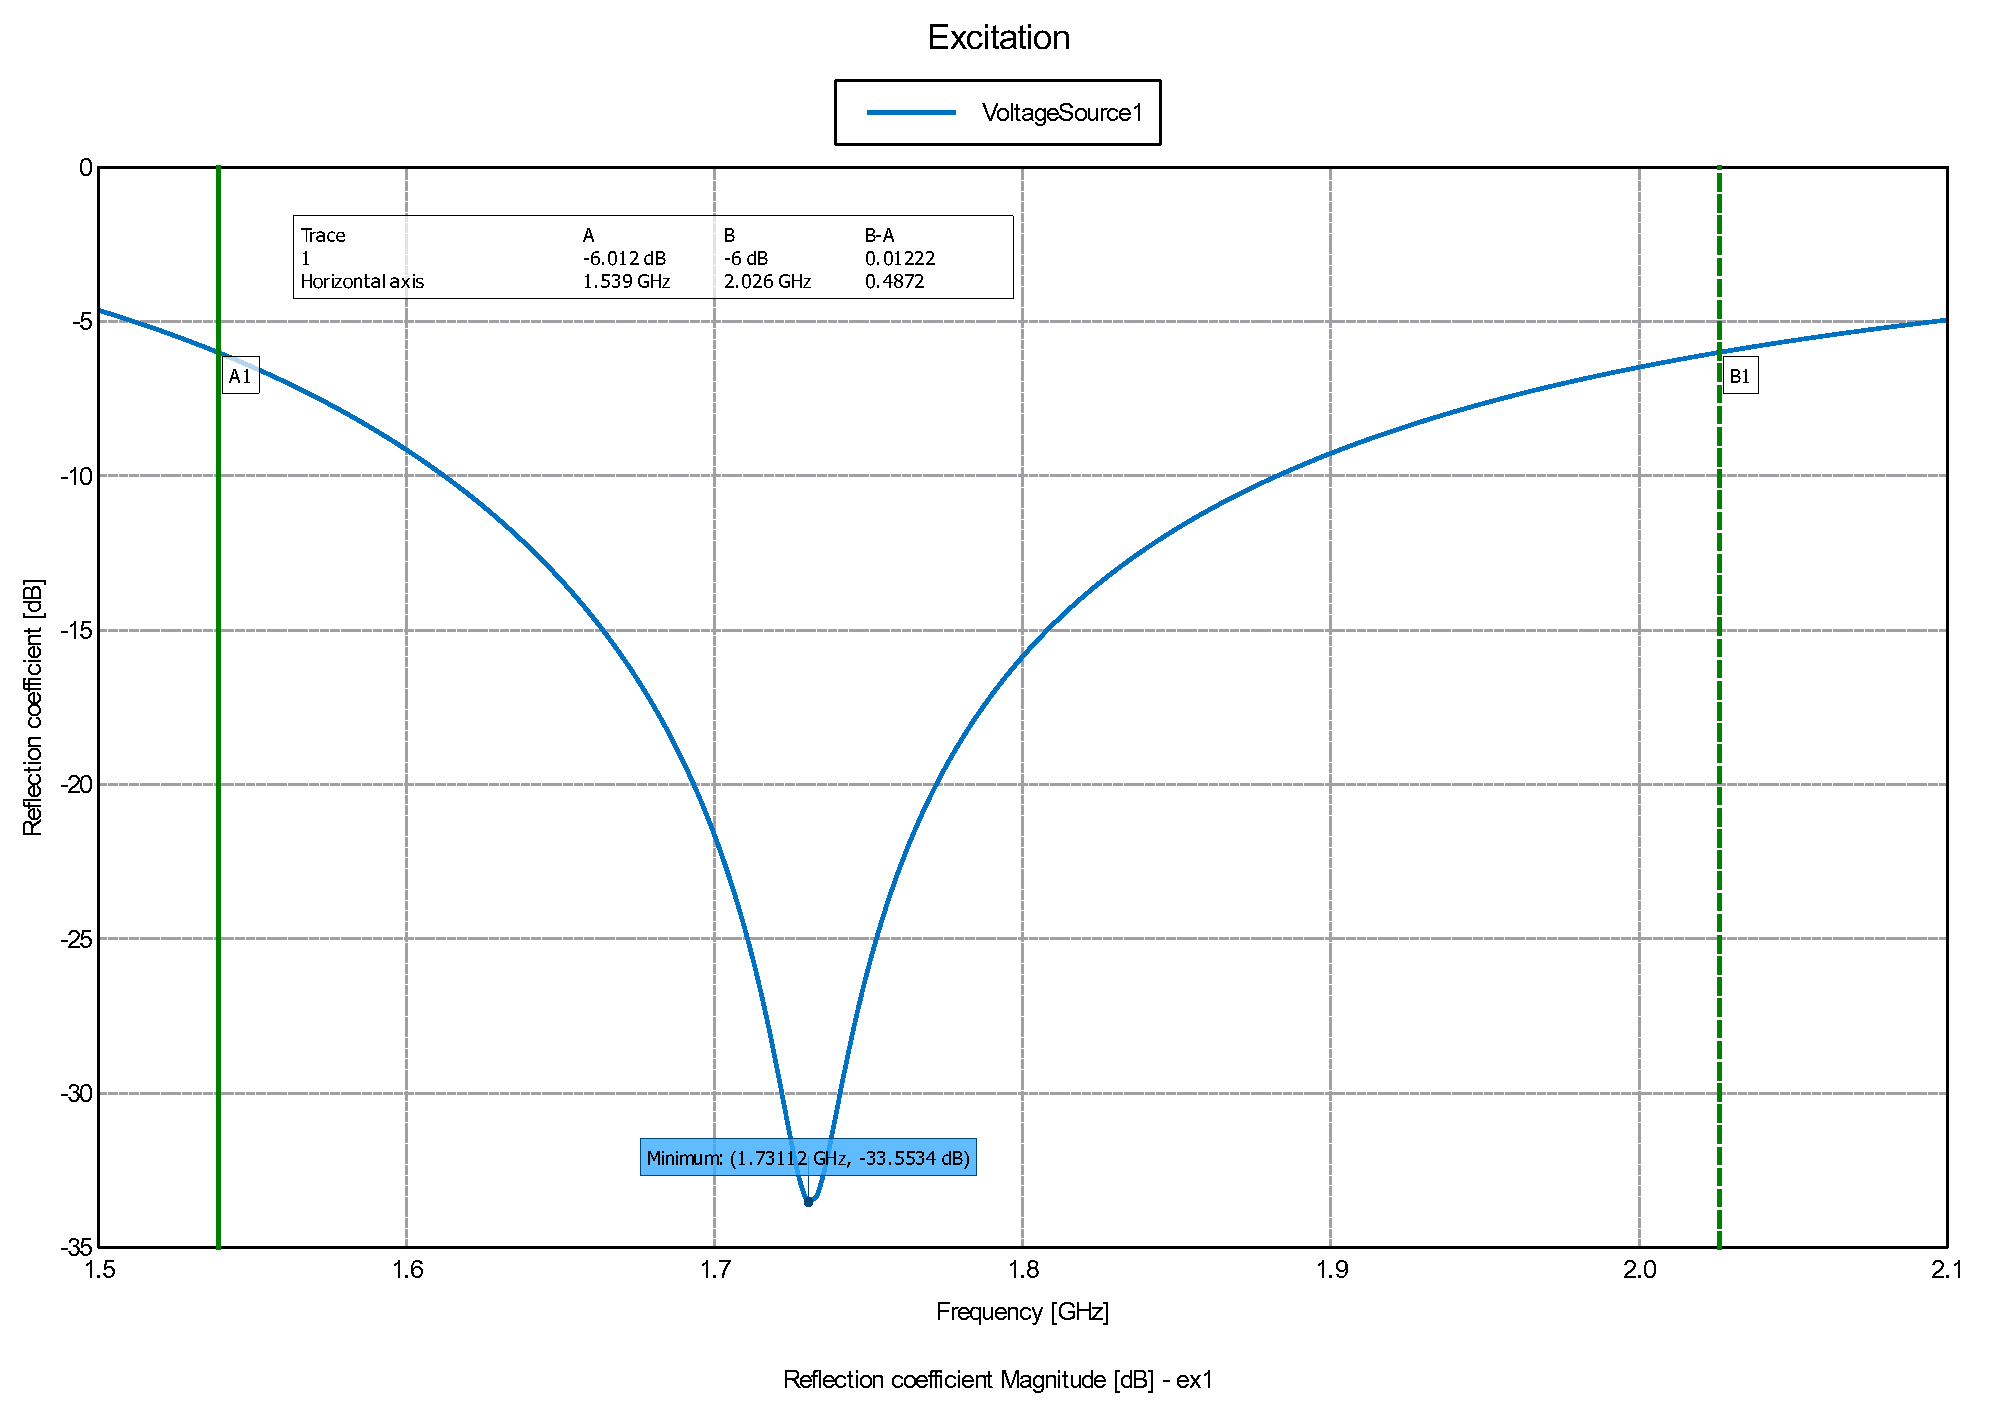
\includegraphics[width = \textwidth]{gamma5022.pdf}
  \caption{$\Gamma_L$  en fonction de la fréquence de l'antenne dipôle adaptée pour \SI{1.8}{\giga\hertz}, et diamètre multiplié par 50.\label{fig:gamma5022}}
\end{figure}
On constate en effet que la largeur de bande passe de \SI{225}{\mega\hertz} (figure \ref{fig:gamma22}) à \SI{487}{\mega\hertz} (figure \ref{fig:gamma5022}). Ceci s'explique par le fait qu'augmenter le diamètre du fil réduit la pente de $\Im(Z_L)$ en fonction de la fréquence.

\subsection{Le dipôle replié}
Le coefficient de réflexion du dipôle demi-onde replié est représenté en fonction de la fréquence à la figure \ref{fig:Z231}.

\begin{figure}[htbp]
  \centering
  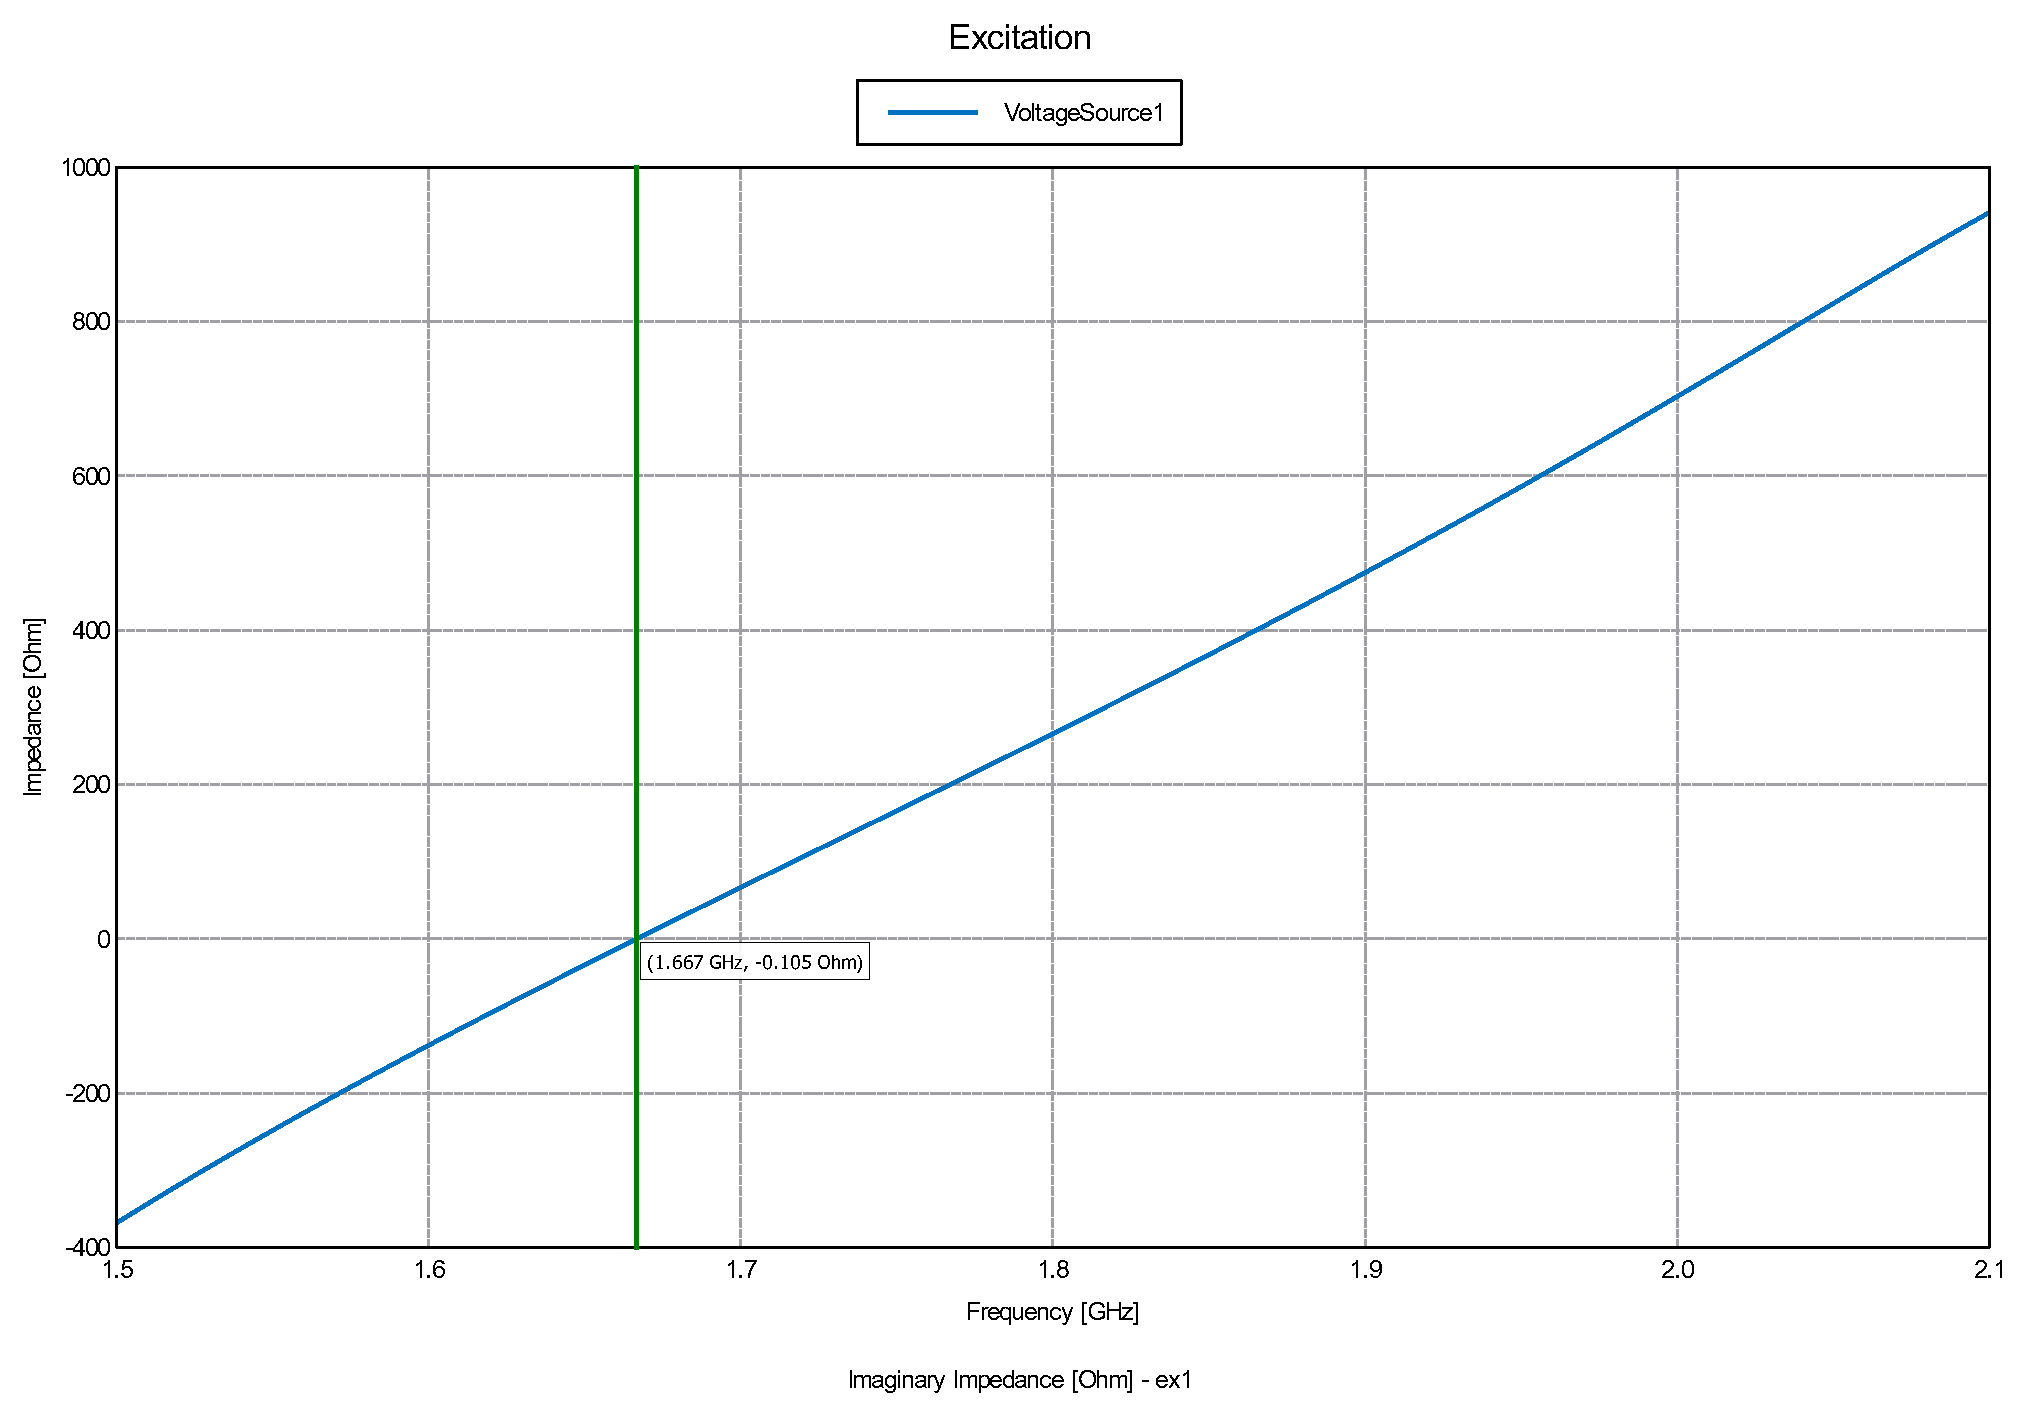
\includegraphics[width = \textwidth]{Z231.pdf}
  \caption{$\Im(Z_L)$ du dipôle demi-onde replié en fonction de la fréquence.\label{fig:Z231}}
\end{figure}
On constate que $\Im(Z_L)$ s'annule maintenant à $f = \SI{1.67}{\giga\hertz}$. Puisque $\Im(Z_L)$ évolue linéairement avec la fréquence, il suffit de remplacer le paramètre $\lambda$ dans le dimensionnement de l'antenne par $\frac{1.67}{1.8}\lambda$ pour construire un dipôle replié qui résonne effectivement autour de \SI{1.8}{\giga\hertz}. Ceci est fait à la figure \ref{fig:Z232}, qui représente la partie imaginaire de l'impédance du dipôle replié de longueur $l = 0.464 \lambda$ en fonction de la fréquence.
\begin{figure}[htbp]
  \centering
  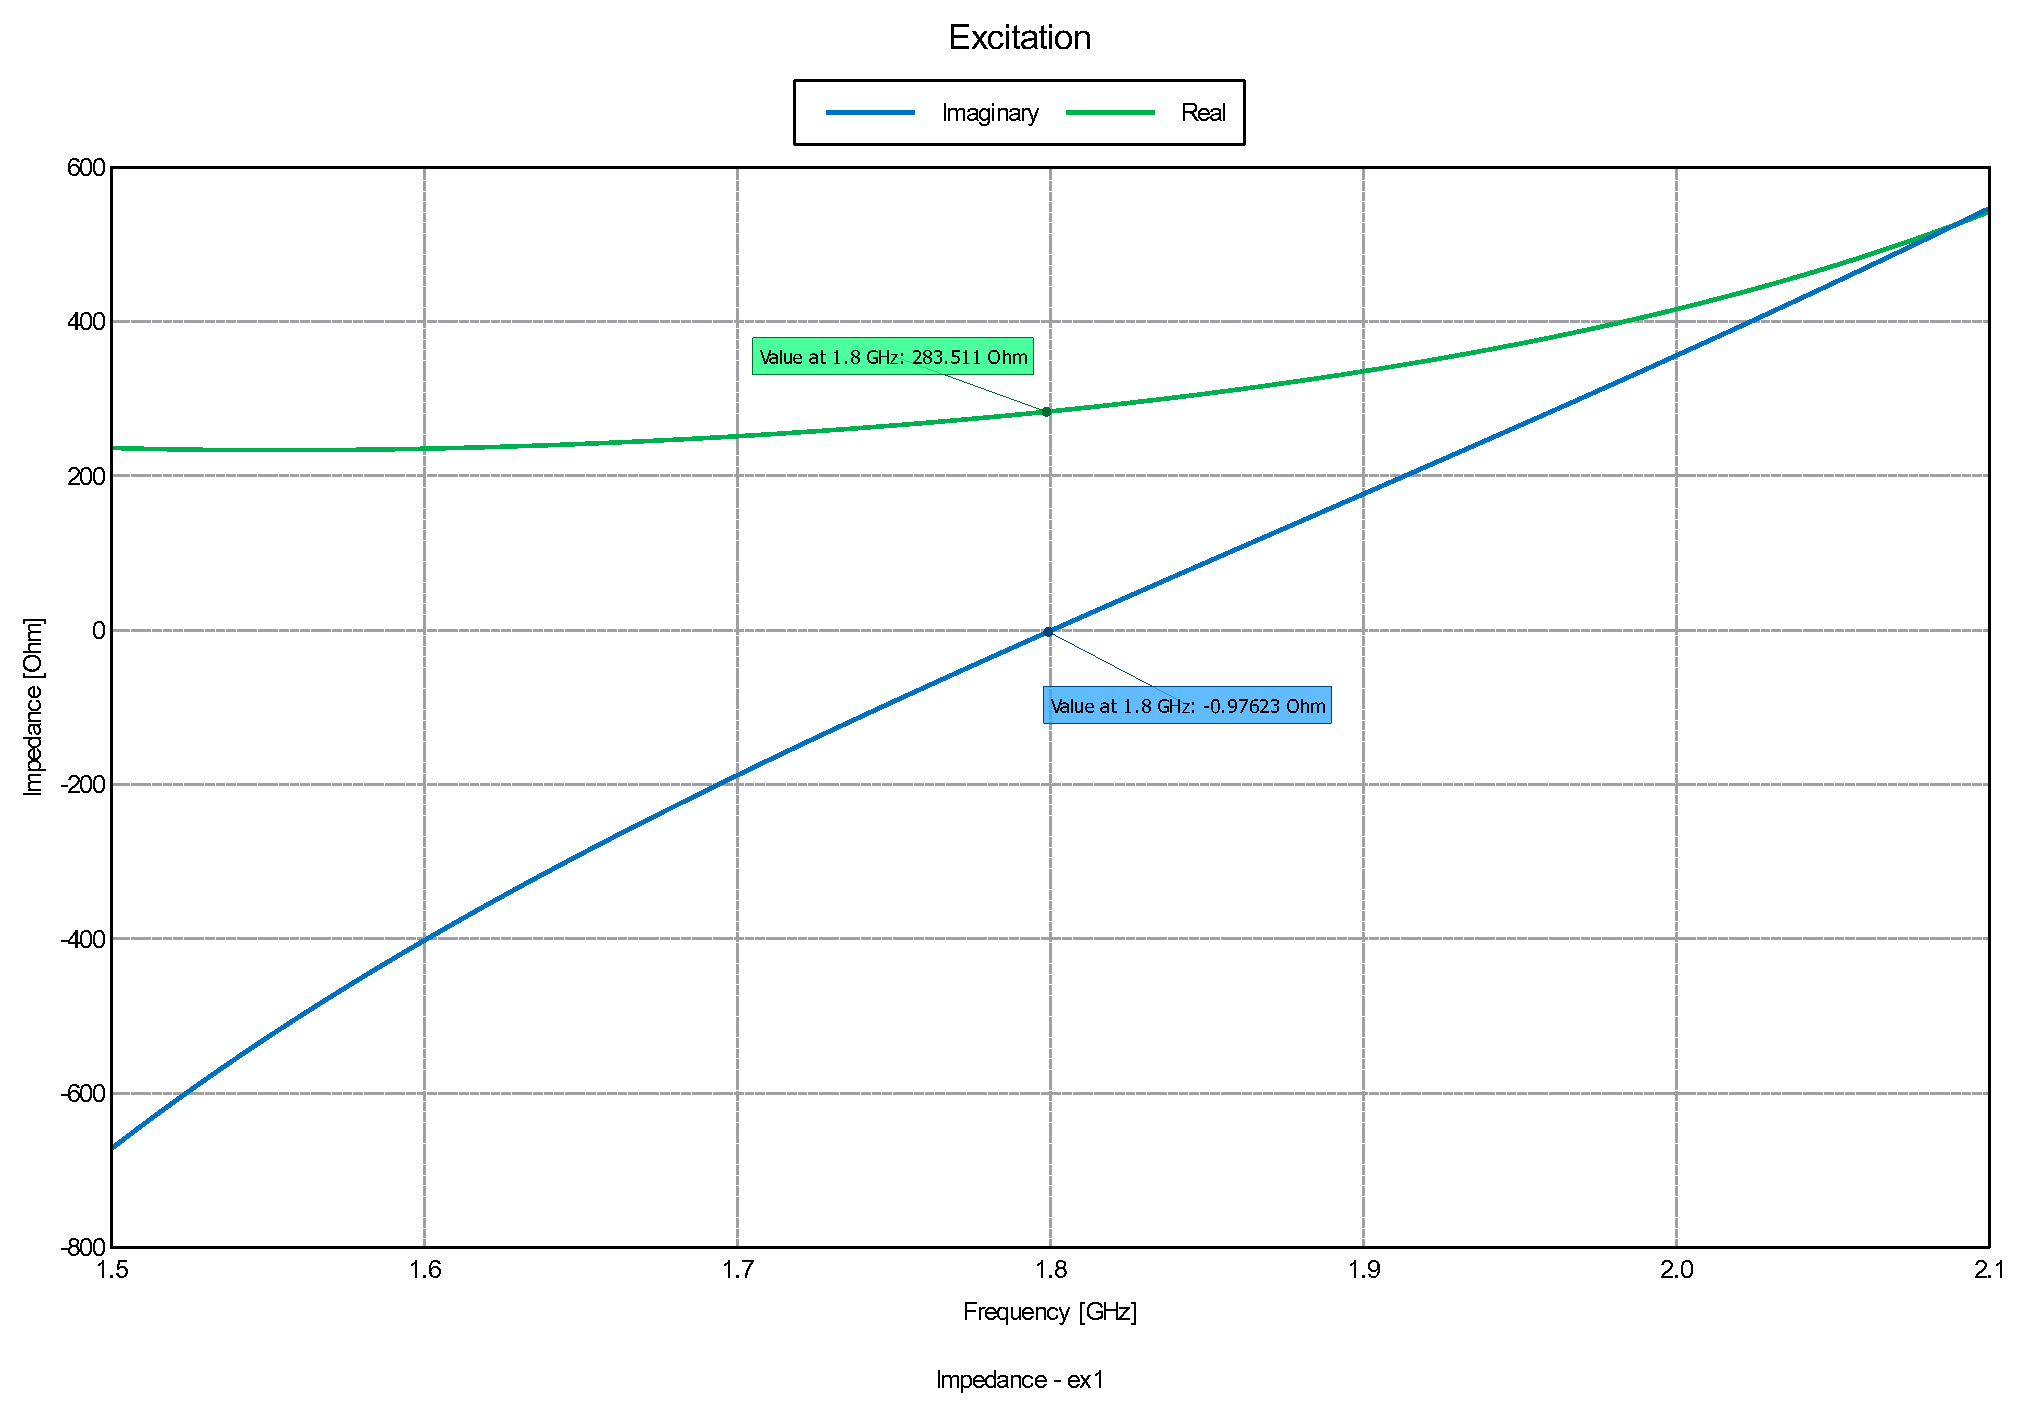
\includegraphics[width = \textwidth]{Z232.pdf}
  \caption{$\Im(Z_L)$ en fonction du dipôle replié adapté pour \SI{1.8}{\giga\hertz}.\label{fig:Z232}}
\end{figure}
Sur la figure \ref{fig:Z232}, on constate aussi que la partie réelle de l'impédance du dipôle replié est près de 4 fois supérieure à la partie réelle de l'impédance du dipôle demi-onde.

Le coefficient de réflexion de ce dipôle replié est représenté en fonction de la fréquence à la figure \ref{fig:gamma23},
\begin{figure}[htbp]
  \centering
  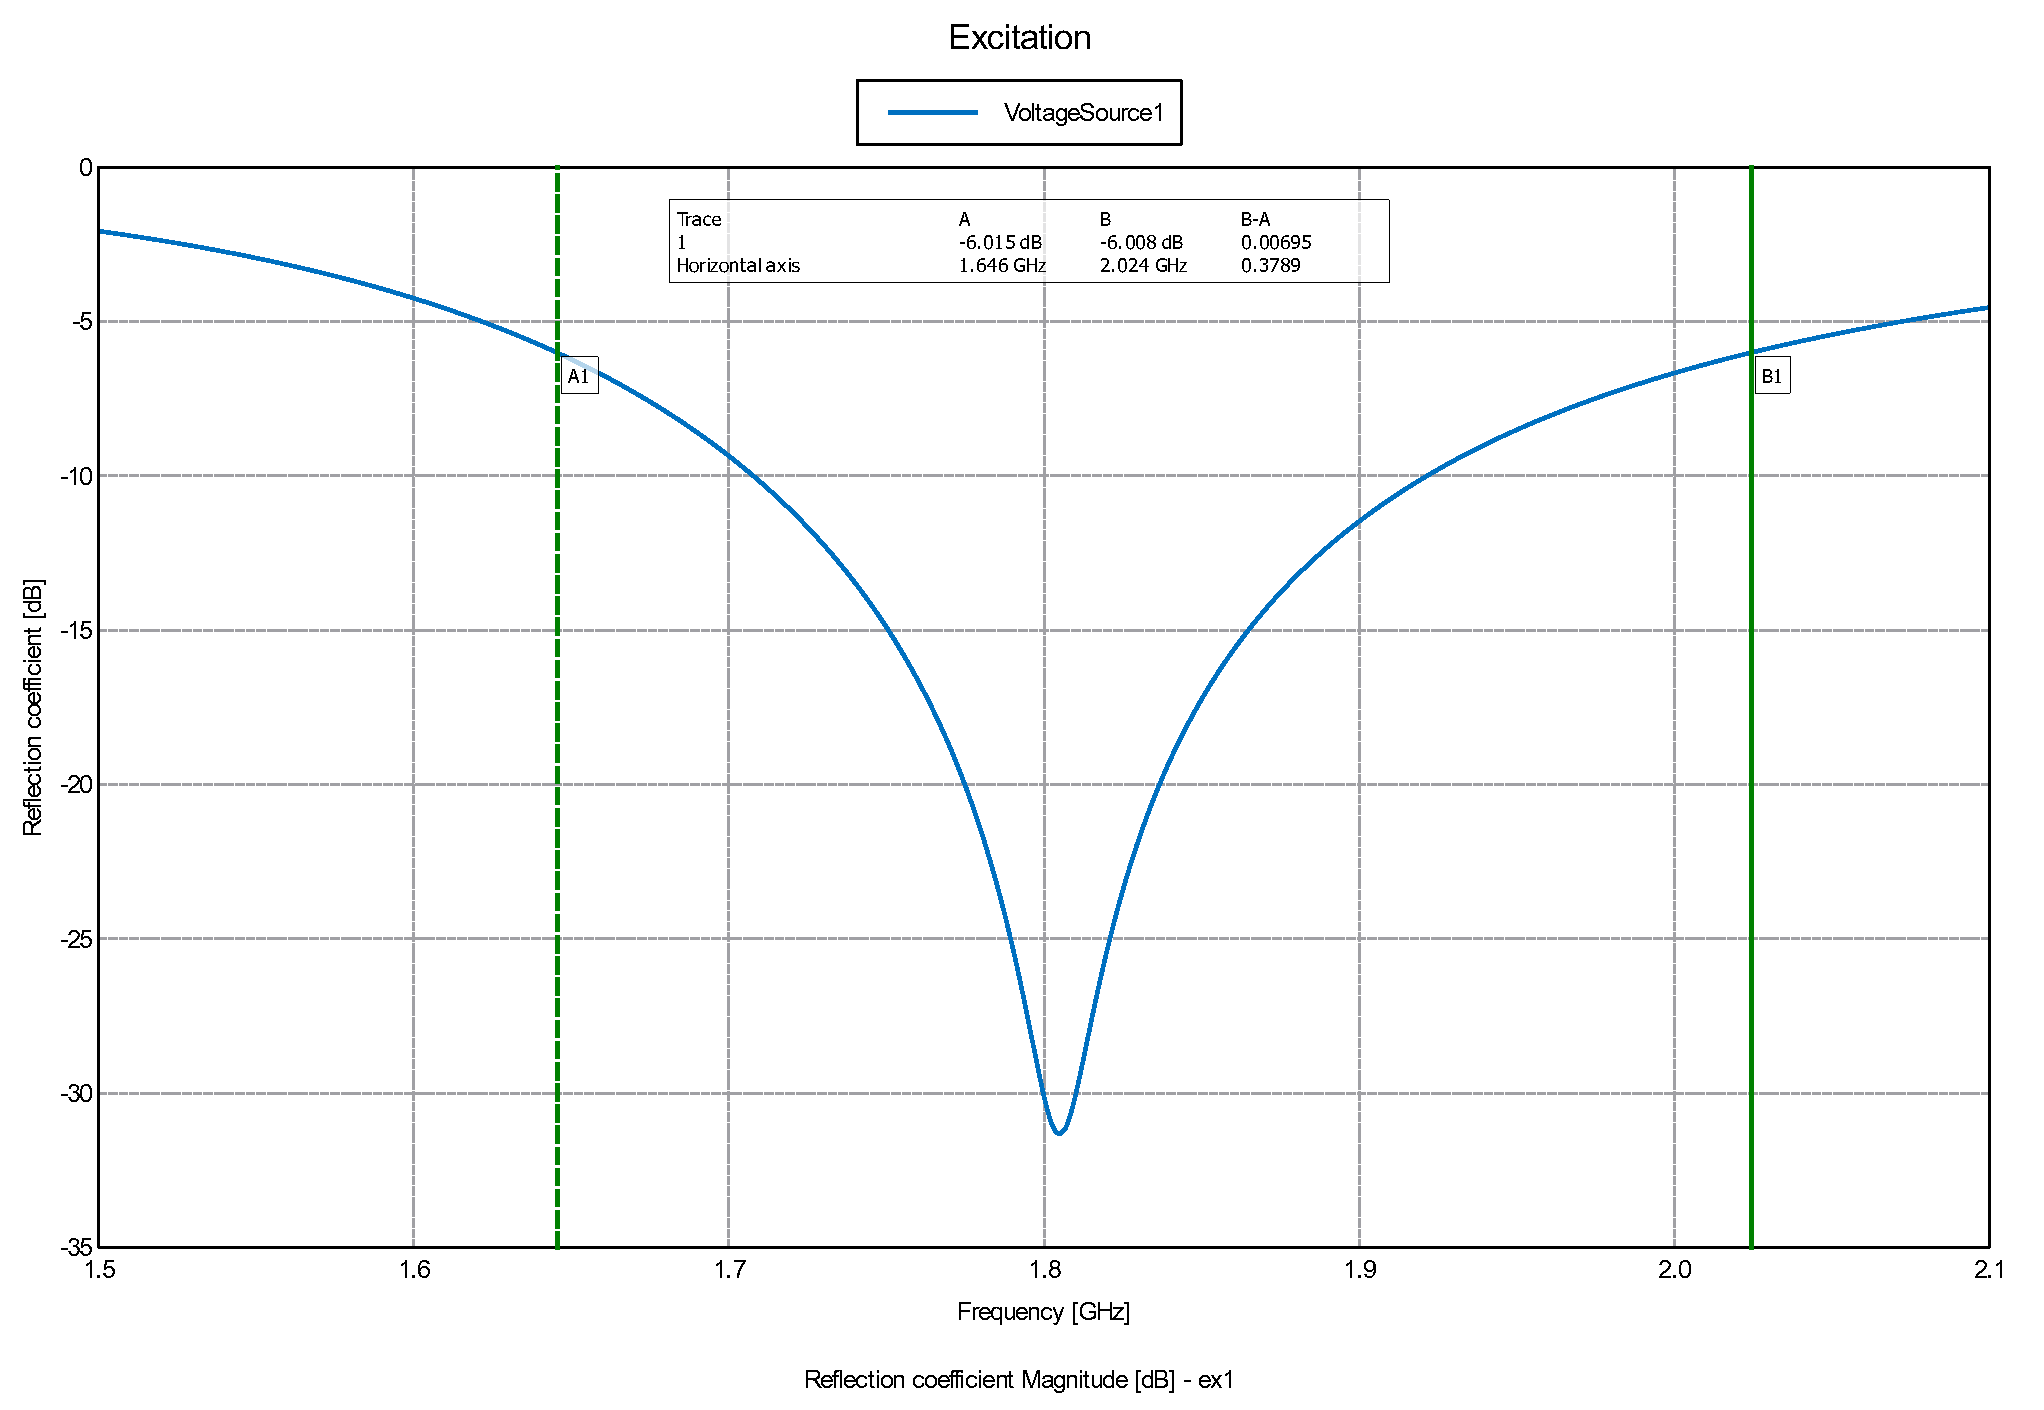
\includegraphics[width = \textwidth]{gamma23.pdf}
  \caption{$\Gamma_L$ du dipôle replié en fonction de la fréquence.\label{fig:gamma23}}
\end{figure}
pour une source d'impédance \SI{300}{\ohm}. Sur cette figure, on lit $\Gamma_L \simeq \SI{-30}{\deci\bel}$ à \SI{1.8}{\giga\hertz} et une largeur de bande de \SI{379}{\mega\hertz}. La largeur de bande à donc augmenté de plus de \SI{50}{\percent} par rapport à celle du dipôle demi-onde de même diamètre ($0.00001\lambda$).

Le gain est représenté dans un diagramme polaire à la figure \ref{fig:gain234}.
\begin{figure}[htbp]
  \centering
  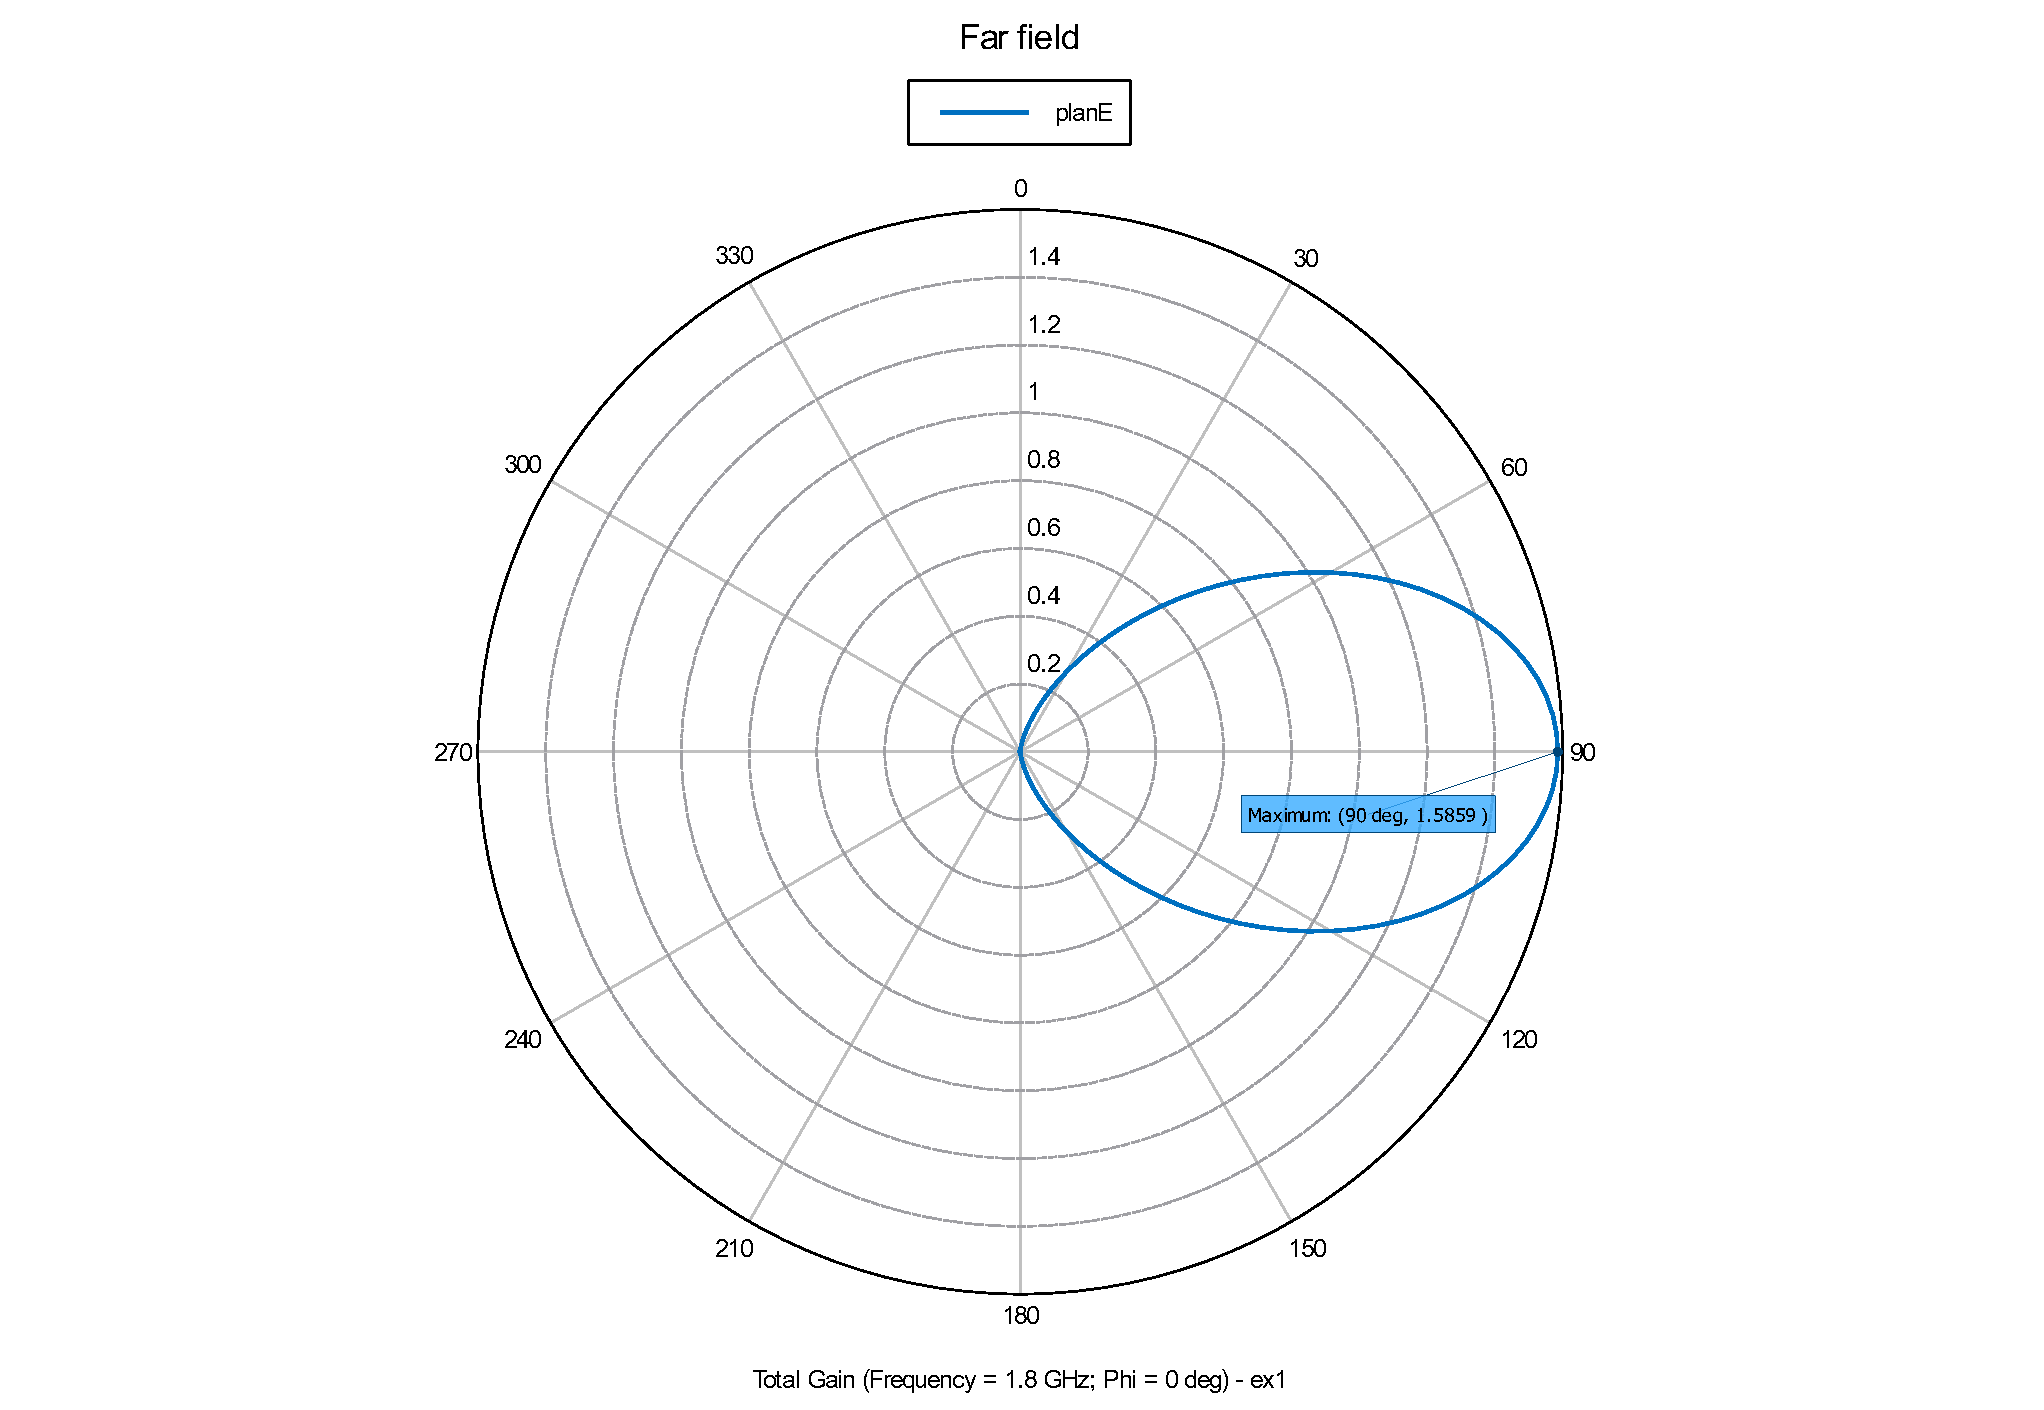
\includegraphics[width = \textwidth]{gain234.pdf}
  \caption{Diagramme polaire du gain du dipôle replié dans le plan E.\label{fig:gain234}}
\end{figure}
Le gain maximal est toujours bien évidemment dans le plan $\theta = 0$ et vaut \num{1.56}, ce qui est légèrement inférieur au gain maximal du dipôle demi-onde.

\subsection{Réseau de dipôles}
Nous étudions ici un réseau de 4 dipôles demi-onde dont la longueur est telle que $\Im(Z_L)=0$ (voir section \ref{subsec:demionde}), et alignés verticalement. Pour avoir une directivité maximale de rayonnement en $\theta=\frac{2\pi}{3}$, on peut calculer le déphasage nécessaire entre chaque source par la relation \ref{eqn:dephasage}.
\begin{equation}\label{eqn:dephasage}
\delta = \beta d \cos(\theta)
\end{equation}
Où $\beta = \frac{2\pi f}{c}$ est le nombre d'onde et $d$, la distance entre deux sources.
Le système est ensuite simulé : on peut constater sur la figure \ref{fig:rayonnement4} que le gain maximum est de $\num{4.24} = \SI{6.27}{\deci\bel}$.
\begin{figure}[htbp]
  \centering
  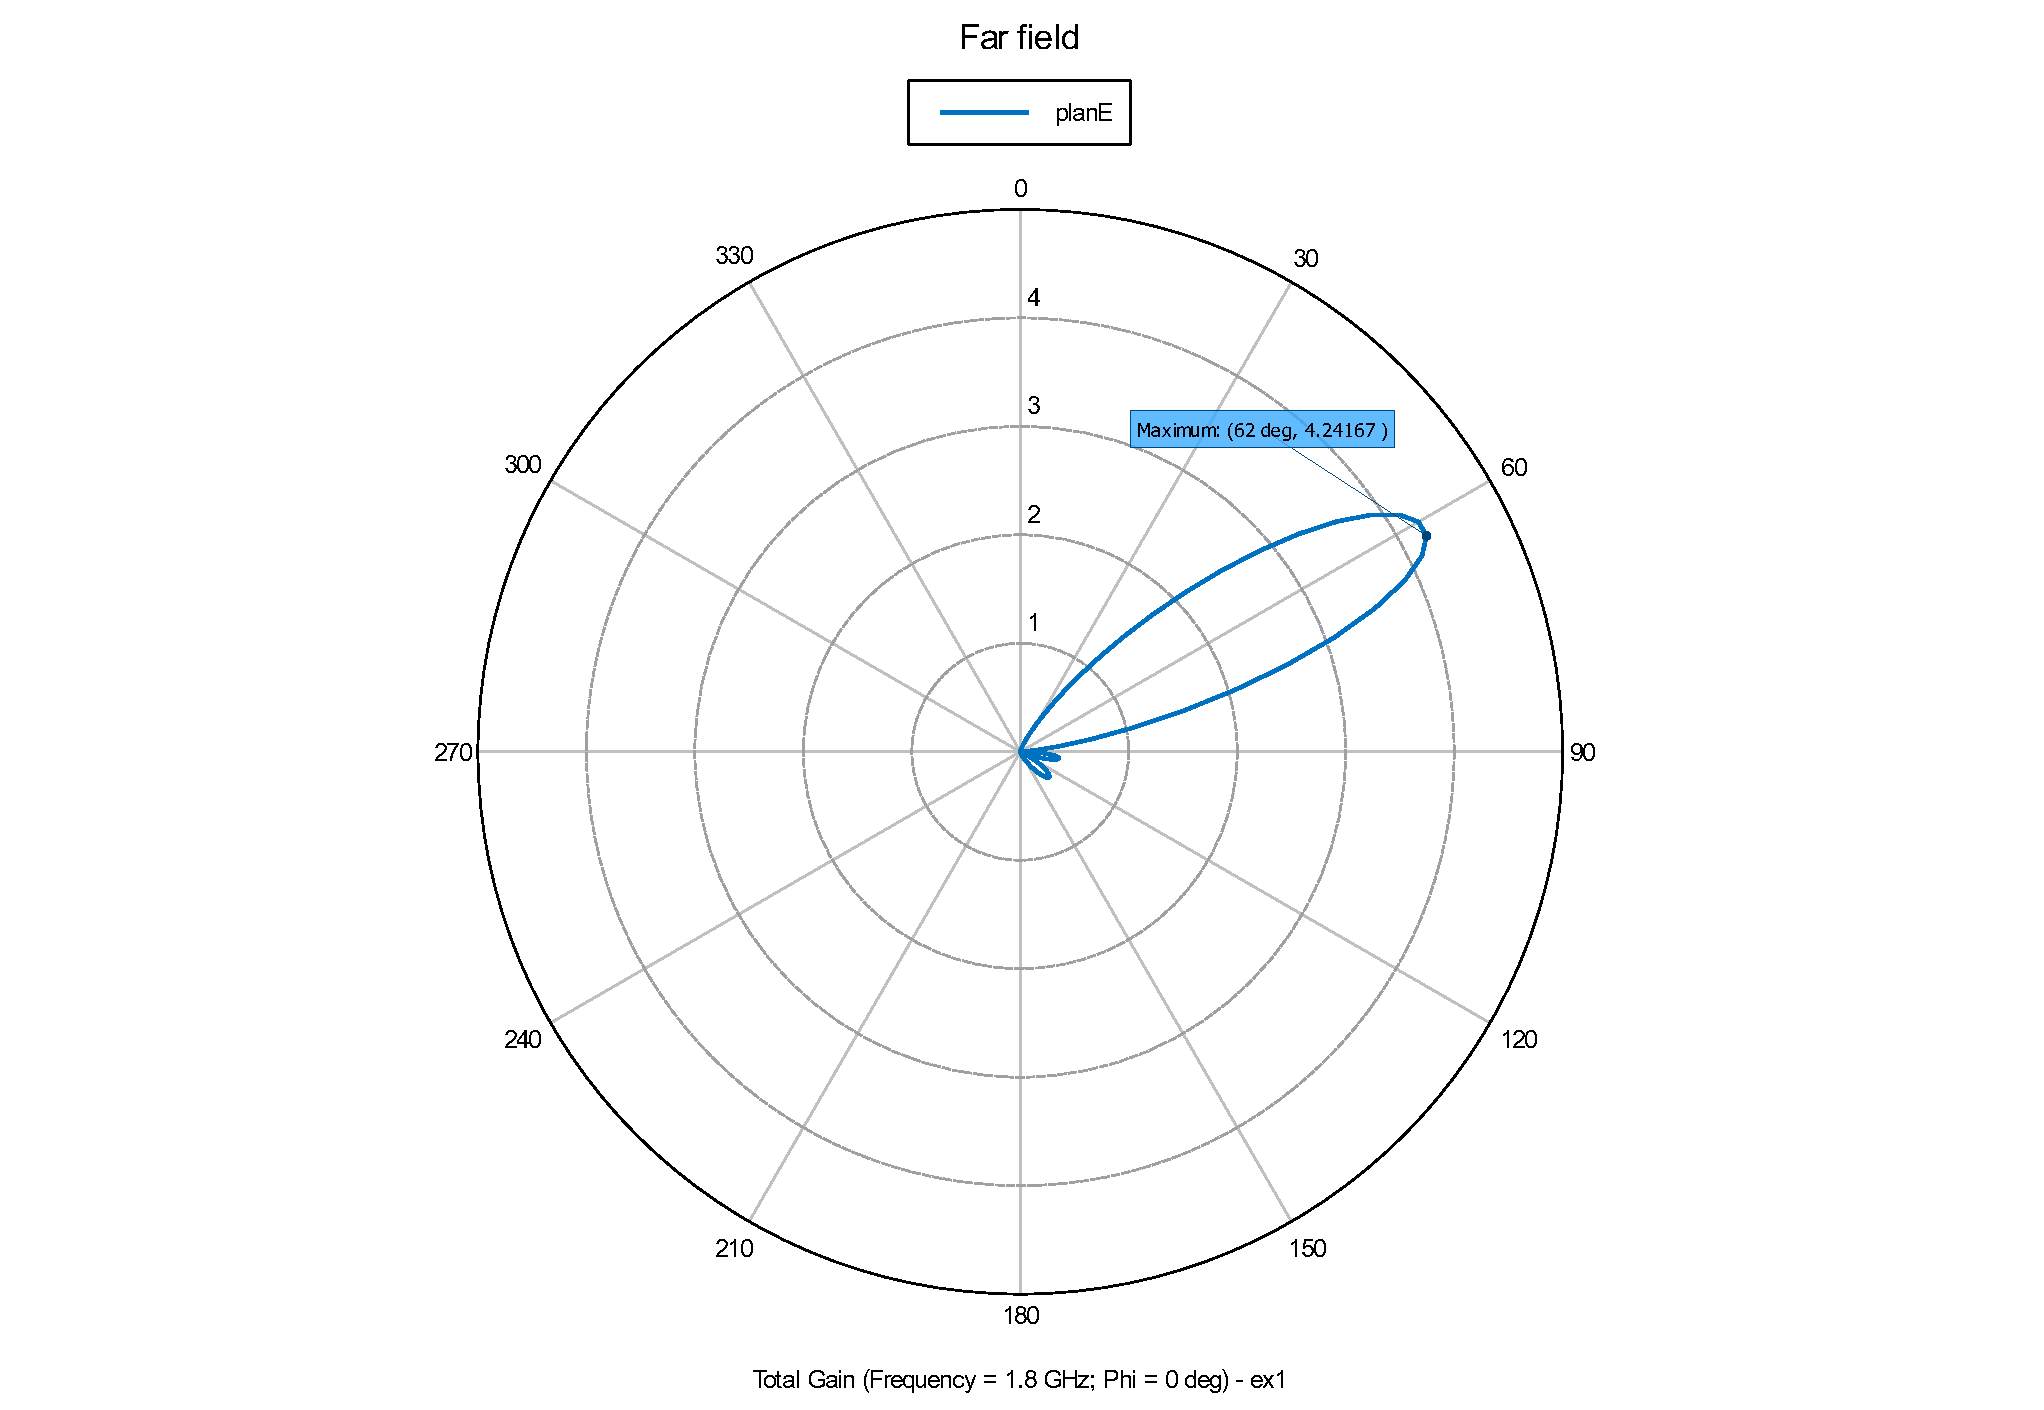
\includegraphics[width = \textwidth]{rayonnement24.pdf}
  \caption{Diagramme de rayonnement du réseau de dipôles demi-onde dans le plan E\label{fig:rayonnement4}}
\end{figure}

Nous avons ensuite rajouté au système un plan conducteur parfait de dimension $3\lambda \times \lambda$ parallèle à l'axe des dipôles et à une distance $\frac{\lambda}{4}$ de ceux-ci. Après une seconde simulation, on peut constater un gain de $\num{14} = \SI{11.46}{\deci\bel}$ sur la figure \ref{fig:rayonnement4reflecteur}, ce qui est nettement mieux que sans le plan réflecteur.
\begin{figure}[htbp]
  \centering
  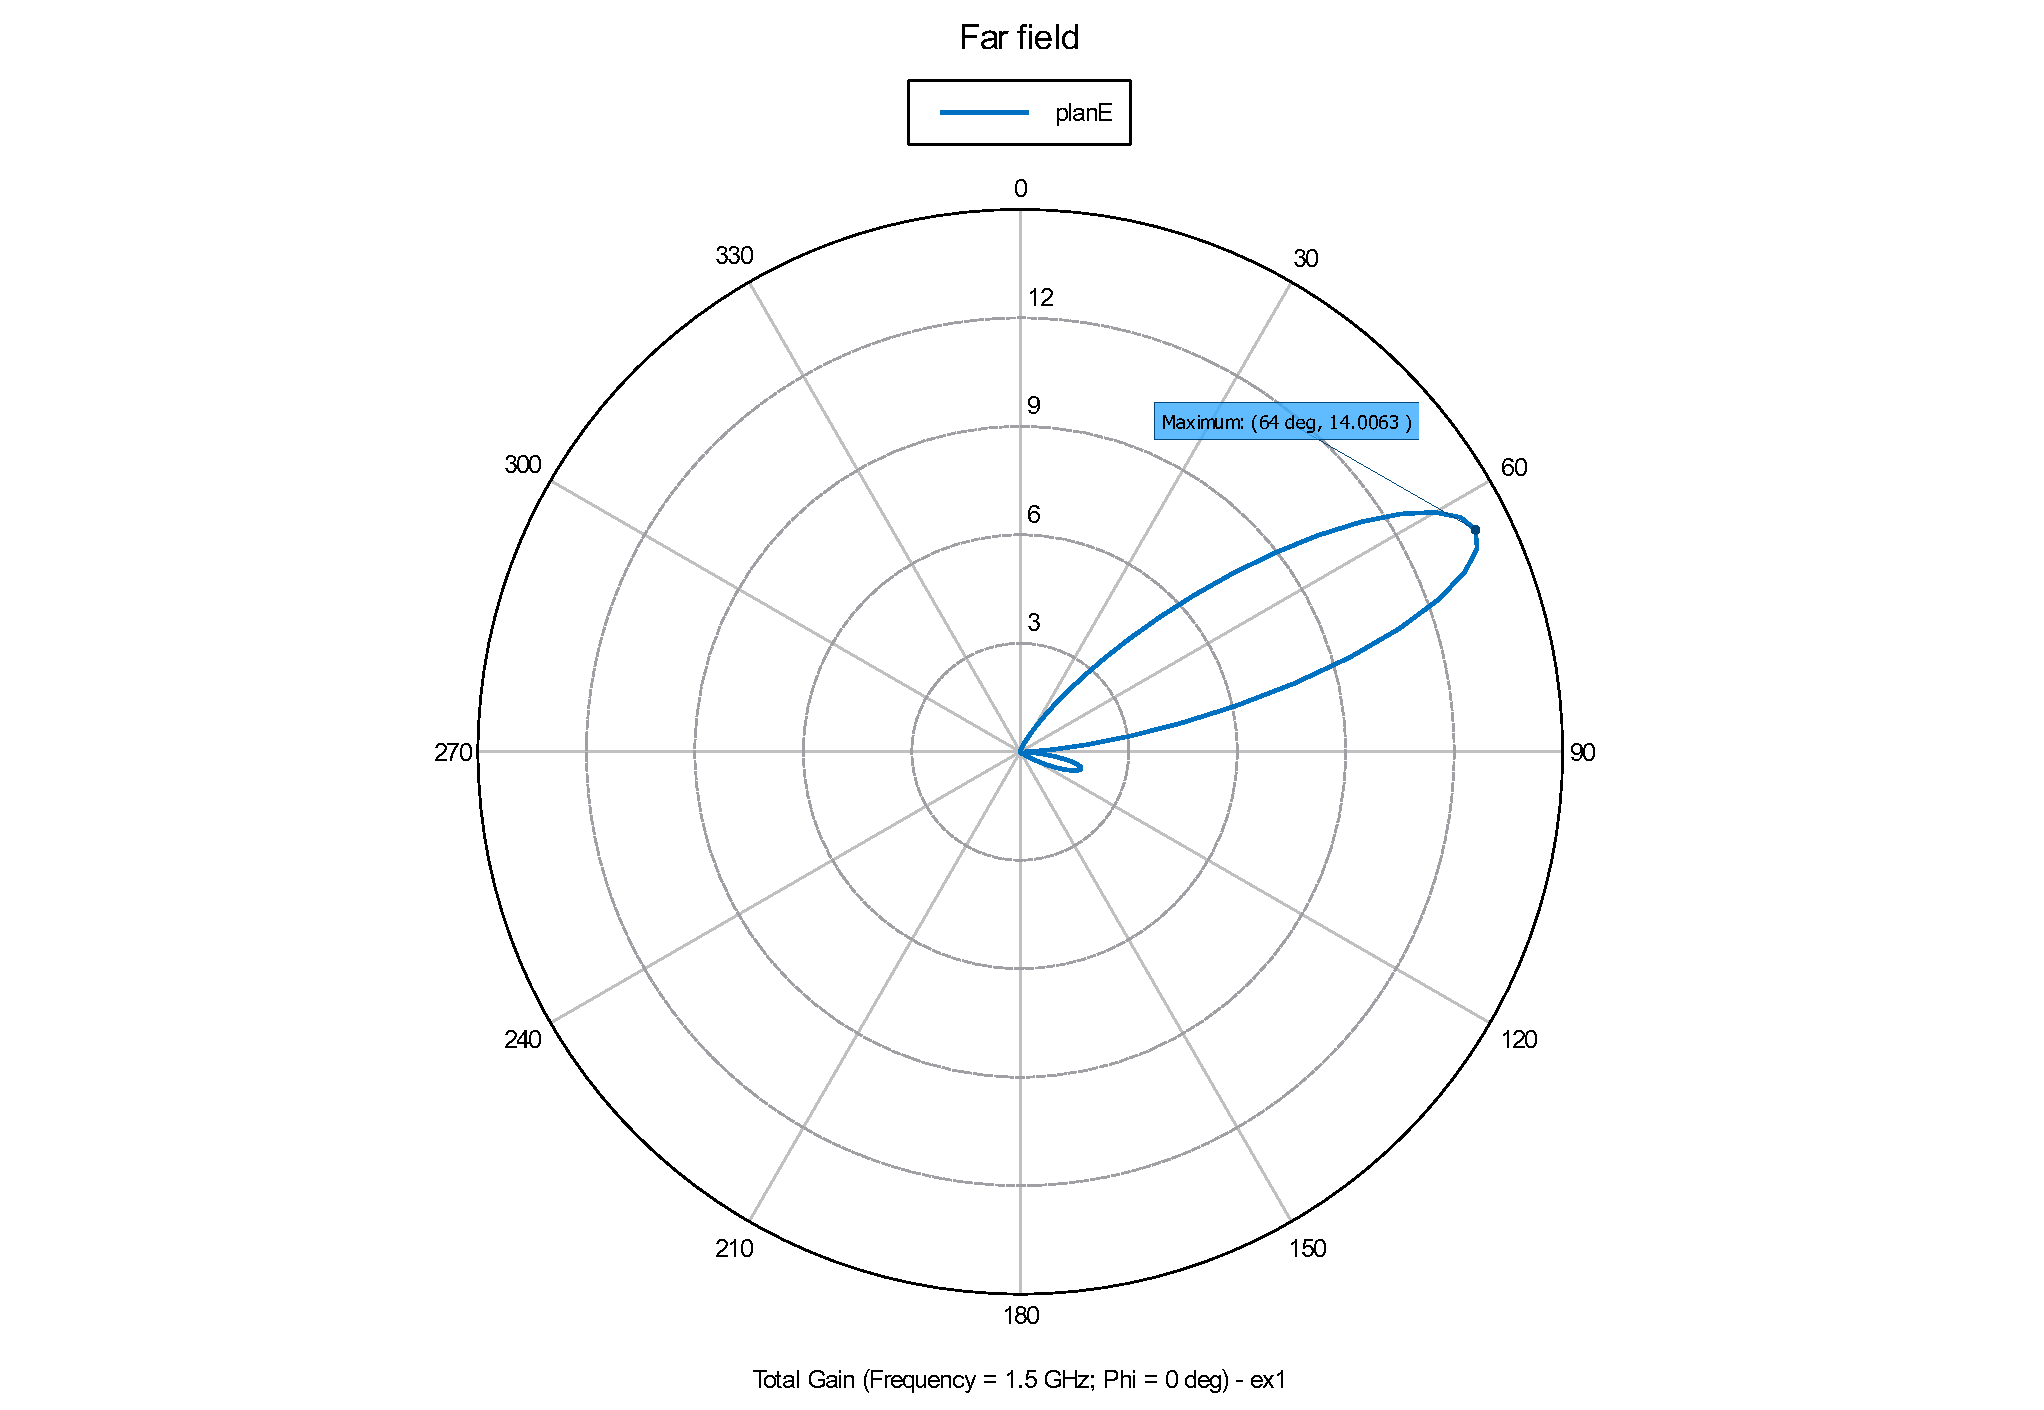
\includegraphics[width = \textwidth]{rayonnement24b.pdf}
  \caption{Diagramme de rayonnement du réseau de dipôles demi-onde avec un plan réflecteur dans le plan E\label{fig:rayonnement4reflecteur}}
\end{figure}

Ceci peut facilement s'expliquer par le fait que l'onde est réfléchie sur le plan conducteur et crée une interférence constructrice avec l'onde émise dans le sens opposé par le dipôle. On voit donc ici que le plan doit être écarté de $\frac{\lambda}{4}$ pour assurer que l'interférence soit bien constructive. En effet, l'onde réfléchie doit parcourir $\frac{\lambda}{2}$ en plus que l'onde originale, ce qui correspond à un déphasage de $\pi$. A ceci s'ajoute le déphasage induit par la réflexion d'une onde polarisée parallèlement qui est lui aussi de $\pi$. Le déphasage total est donc de $2\pi$, ce qui est souhaité. Tous les plans placés à $(2k+1)\frac{\lambda}{4} \; (k \in \mathbb{N})$ satisfont cette condition, mais on choisit le plus proche afin de réfléchir le plus d'énergie possible.

Finalement, les trois configurations: dipôle demi-onde, dipôle replié et réseau de dipôles sont comparés à la table \ref{tbl:comp}.
\begin{table}[htbp]
\begin{tabular}{ccc}
  \hline
       Dipôle demi-onde & Réseau sans réflecteur & Réseau avec réflecteur \\
  \hline
  $\SI{1.79}{\deci\bel}$ & $\SI{6.27}{\deci\bel}$ & $\SI{11.46}{\deci\bel}$ \\
  \hline
\end{tabular}
\caption{Comparaison des gains maximum des trois configurations d'antennes dipôles.\label{tbl:comp}}
\end{table}

%Coucou jason! Attention qu'une ligne vide = 1 nouveau paragraphe=> une idée séparée. Si tu veux absolument mettre des lignes vides autour de figures dans le code, mets les en commentaire.

%Kikou nathou ! ok mais je vois pas trop quelles séparations clochent
